\documentclass[article]{jss}
\usepackage{listings}
\usepackage{bm}
\usepackage{float}
\floatstyle{ruled}
\newfloat{algorithm}{tbp}{loa}
\floatname{algorithm}{Algorithm}


%%%%%%%%%%%%%%%%%%%%%%%%%%%%%%
%% declarations for jss.cls %%
%%%%%%%%%%%%%%%%%%%%%%%%%%%%%%

%% almost as usual
\author{C. M. Strickland\\Queensland University\\ of Technology \And 
        R. J. Denham\\Department of \\Environment and\\ Resource Management \And
        C. L. Alston\\Queensland University\\ of Technology \And 
        K. L. Mengersen\\Queensland University\\ of Technology}

\title{\pkg{PyMCMC}: A \proglang{Python} Package for Bayesian Estimation 
  Using Markov Chain Monte Carlo}

%% for pretty printing and a nice hypersummary also set:
\Plainauthor{C. M. Strickland, R. J. Denham, C. L. Alston, K. L. Mengersen}
\Plaintitle{PyMCMC: A Python package for Bayesian estimation using Markov chain Monte Carlo}
%\Shorttitle{A Capitalized Title}

%% an abstract and keywords
\Abstract{ 

  Markov chain Monte Carlo (MCMC) estimation provides a solution to
  the complex integration problems that are faced in the Bayesian
  analysis of statistical problems.  The implementation of MCMC
  algorithms is, however, code intensive and time consuming.  We have
  developed a \proglang{Python} package, which is called \pkg{PyMCMC},
  that aids in the construction of MCMC samplers and helps to
  substantially reduce the likelihood of coding error, as well as aid
  in the minimisation of repetitive code.  \pkg{PyMCMC} contains
  classes for Gibbs, Metropolis Hastings, independent Metropolis
  Hastings, random walk Metropolis Hastings, orientational bias Monte
  Carlo and slice samplers as well as specific modules for common
  models such as a module for Bayesian regression analysis.
  \pkg{PyMCMC} is straightforward to optimise, taking advantage of the
  \proglang{Python} libraries \pkg{Numpy} and \pkg{Scipy}, as well as being
  readily extensible with \proglang{C} or \proglang{Fortran}.

}

\Keywords{MCMC, Metropolis Hastings, Gibbs, Bayesian, OBMC, slice sampler, \proglang{Python}}
\Plainkeywords{MCMC, Metropolis Hastings, Gibbs, Bayesian, OBMC, slice sampler, Python} 


%% publication information
%% NOTE: Typically, this can be left commented and will be filled out by the technical editor
%% \Volume{13}
%% \Issue{9}
%% \Month{September}
%% \Year{2004}
%% \Submitdate{2004-09-29}
%% \Acceptdate{2004-09-29}

%% The address of (at least) one author should be given
%% in the following format:
\Address{
  C. M. Strickland\\
  Mathematical Sciences\\
  GPO Box 2434\\
  Queensland University of Technology\\
  Queensland, 4001, Australia\\
  E-mail: \email{ christopher.strickland@qut.edu.au}
}

%% I would put both our affiliations in If I knew how.

% \Address{
%   Robert Denham\\
%   Remote Sensing Centre\\
%   Department of Environment and Resource Management\\
%   GPO Box 2454\\
%   Brisbane,
%   Queensland, 4001, Australia\\
%   E-mail: \email{ robert.denham@derm.qld.gov.au}
% }

%% It is also possible to add a telephone and fax number
%% before the e-mail in the following format:
%% Telephone: +43/1/31336-5053
%% Fax: +43/1/31336-734

%% for those who use Sweave please include the following line (with % symbols):
%% need no \usepackage{Sweave.sty}

%% end of declarations %%%%%%%%%%%%%%%%%%%%%%%%%%%%%%%%%%%%%%%%%%%%%%%



\begin{document}


\section{Introduction}

The most common approach currently used in the estimation of Bayesian
Models is Markov chain Monte Carlo (MCMC). \pkg{PyMCMC} is a
\proglang{Python} module that is designed to simplify the construction
of Markov chain Monte Carlo (MCMC) samplers, without sacrificing
flexibility or performance. \proglang{Python} has extensive scientific
libraries, is easily extensible, has a clean syntax and powerful
programming constructs, making it an ideal programming language to
build an MCMC library; see \citet{Python} for further details on the
programming language \proglang{Python}. It contains objects for the
Gibbs sampler, Metropolis Hastings (MH), independent MH, random walk
MH, orientational bias Monte Carlo (OBMC) as well as the slice
sampler. The user can simply piece together the algorithms required
and can easily include their own modules, where necessary. Along with
the standard algorithms, \pkg{PyMCMC} includes a module for Bayesian
regression analysis. This module can be used for the direct analysis
of linear models, or as a part of an MCMC scheme, where the
conditional posterior has the form of a linear model.  It also
contains a class that can be used along with Gibbs sampler for
Bayesian variable selection.

% \pkg{PyMCMC} is designed to be fully flexible, with respect to MCMC design.
This is important in practice, as MCMC algorithms usually need to
be tailored to the problem of interest in order to ensure good results.
Issues such as block size and parameterisation can have a dramatic
effect on the convergence of MCMC sampling schemes. For instance,
\citet{LuiKongWong1994} show theoretically that jointly sampling
parameters in a Gibbs scheme typically leads to a reduction in correlation
in the associated Markov chain in comparison to individually sampling
parameters. This is demonstrated in practical applications in \citet{CarterKohn1994}
and \citet{KimShephardChib1998}. Reducing the correlation in the
Markov chain enables it to move more freely through the parameter
space and as such enables it to escape from local modes in the posterior
distribution. Parameterisation can also have a dramatic effect on
the convergence of MCMC samplers; see for example \citet{GelfandSahuCarlin1995},
\citet{RobersSahu1997}, \citet{PittShepard1999}, \citet{RobertMengersen1999},
\citet{FruwirthSchnatter2004} and \citet{StricklandMartinForbes2008},
who show that the performance of the sampling schemes can be improved
dramatically with the use of efficient parameterisation.

\pkg{PyMCMC} aims to remove unnecessary repetitive coding and hence
reduce the chance of coding error, and importantly, greatly speed up
the construction of efficient MCMC samplers. This is achieved by
taking advantage of the flexibility of \proglang{Python}, which allows
for the implementation of very general code. Another feature of
\proglang{Python}, which is particularly important, is it is also
extremely easy to include modules from compiled languages such as
\proglang{C} and \proglang{Fortran}. This is important to many
practioners who are forced, by the size and complexity of their
problems, to write their MCMC programs entirely in compiled languages,
such as \proglang{C/C++} and \proglang{Fortran} in order to obtain the
necessary speed for feasible practical analysis. With
\proglang{Python}, the user can simply compile \proglang{Fortran} code
using a module called \pkg{F2py} \citep{F2PY}, or inline \proglang{C}
using \pkg{Weave}, which is a part of \pkg{Scipy} \citep{NumpyScipy},
and use the subroutines directly from \proglang{Python}. \pkg{F2py}
can also be used to directly call \proglang{C} routines with the aid
of \proglang{Fortran} signature file. This enables the use of
\pkg{PyMCMC} and \proglang{Python} as a rapid application development
environment, without comprimising on performance by writing only very
small segments of their own code in a compiled language. It should be
mentioned that for most reasonable sized problems \pkg{PyMCMC} is
sufficiently fast for practical MCMC analysis without the need for
specialised modules.

%
\begin{figure}[t!]
  \begin{center}
\hspace*{-1cm}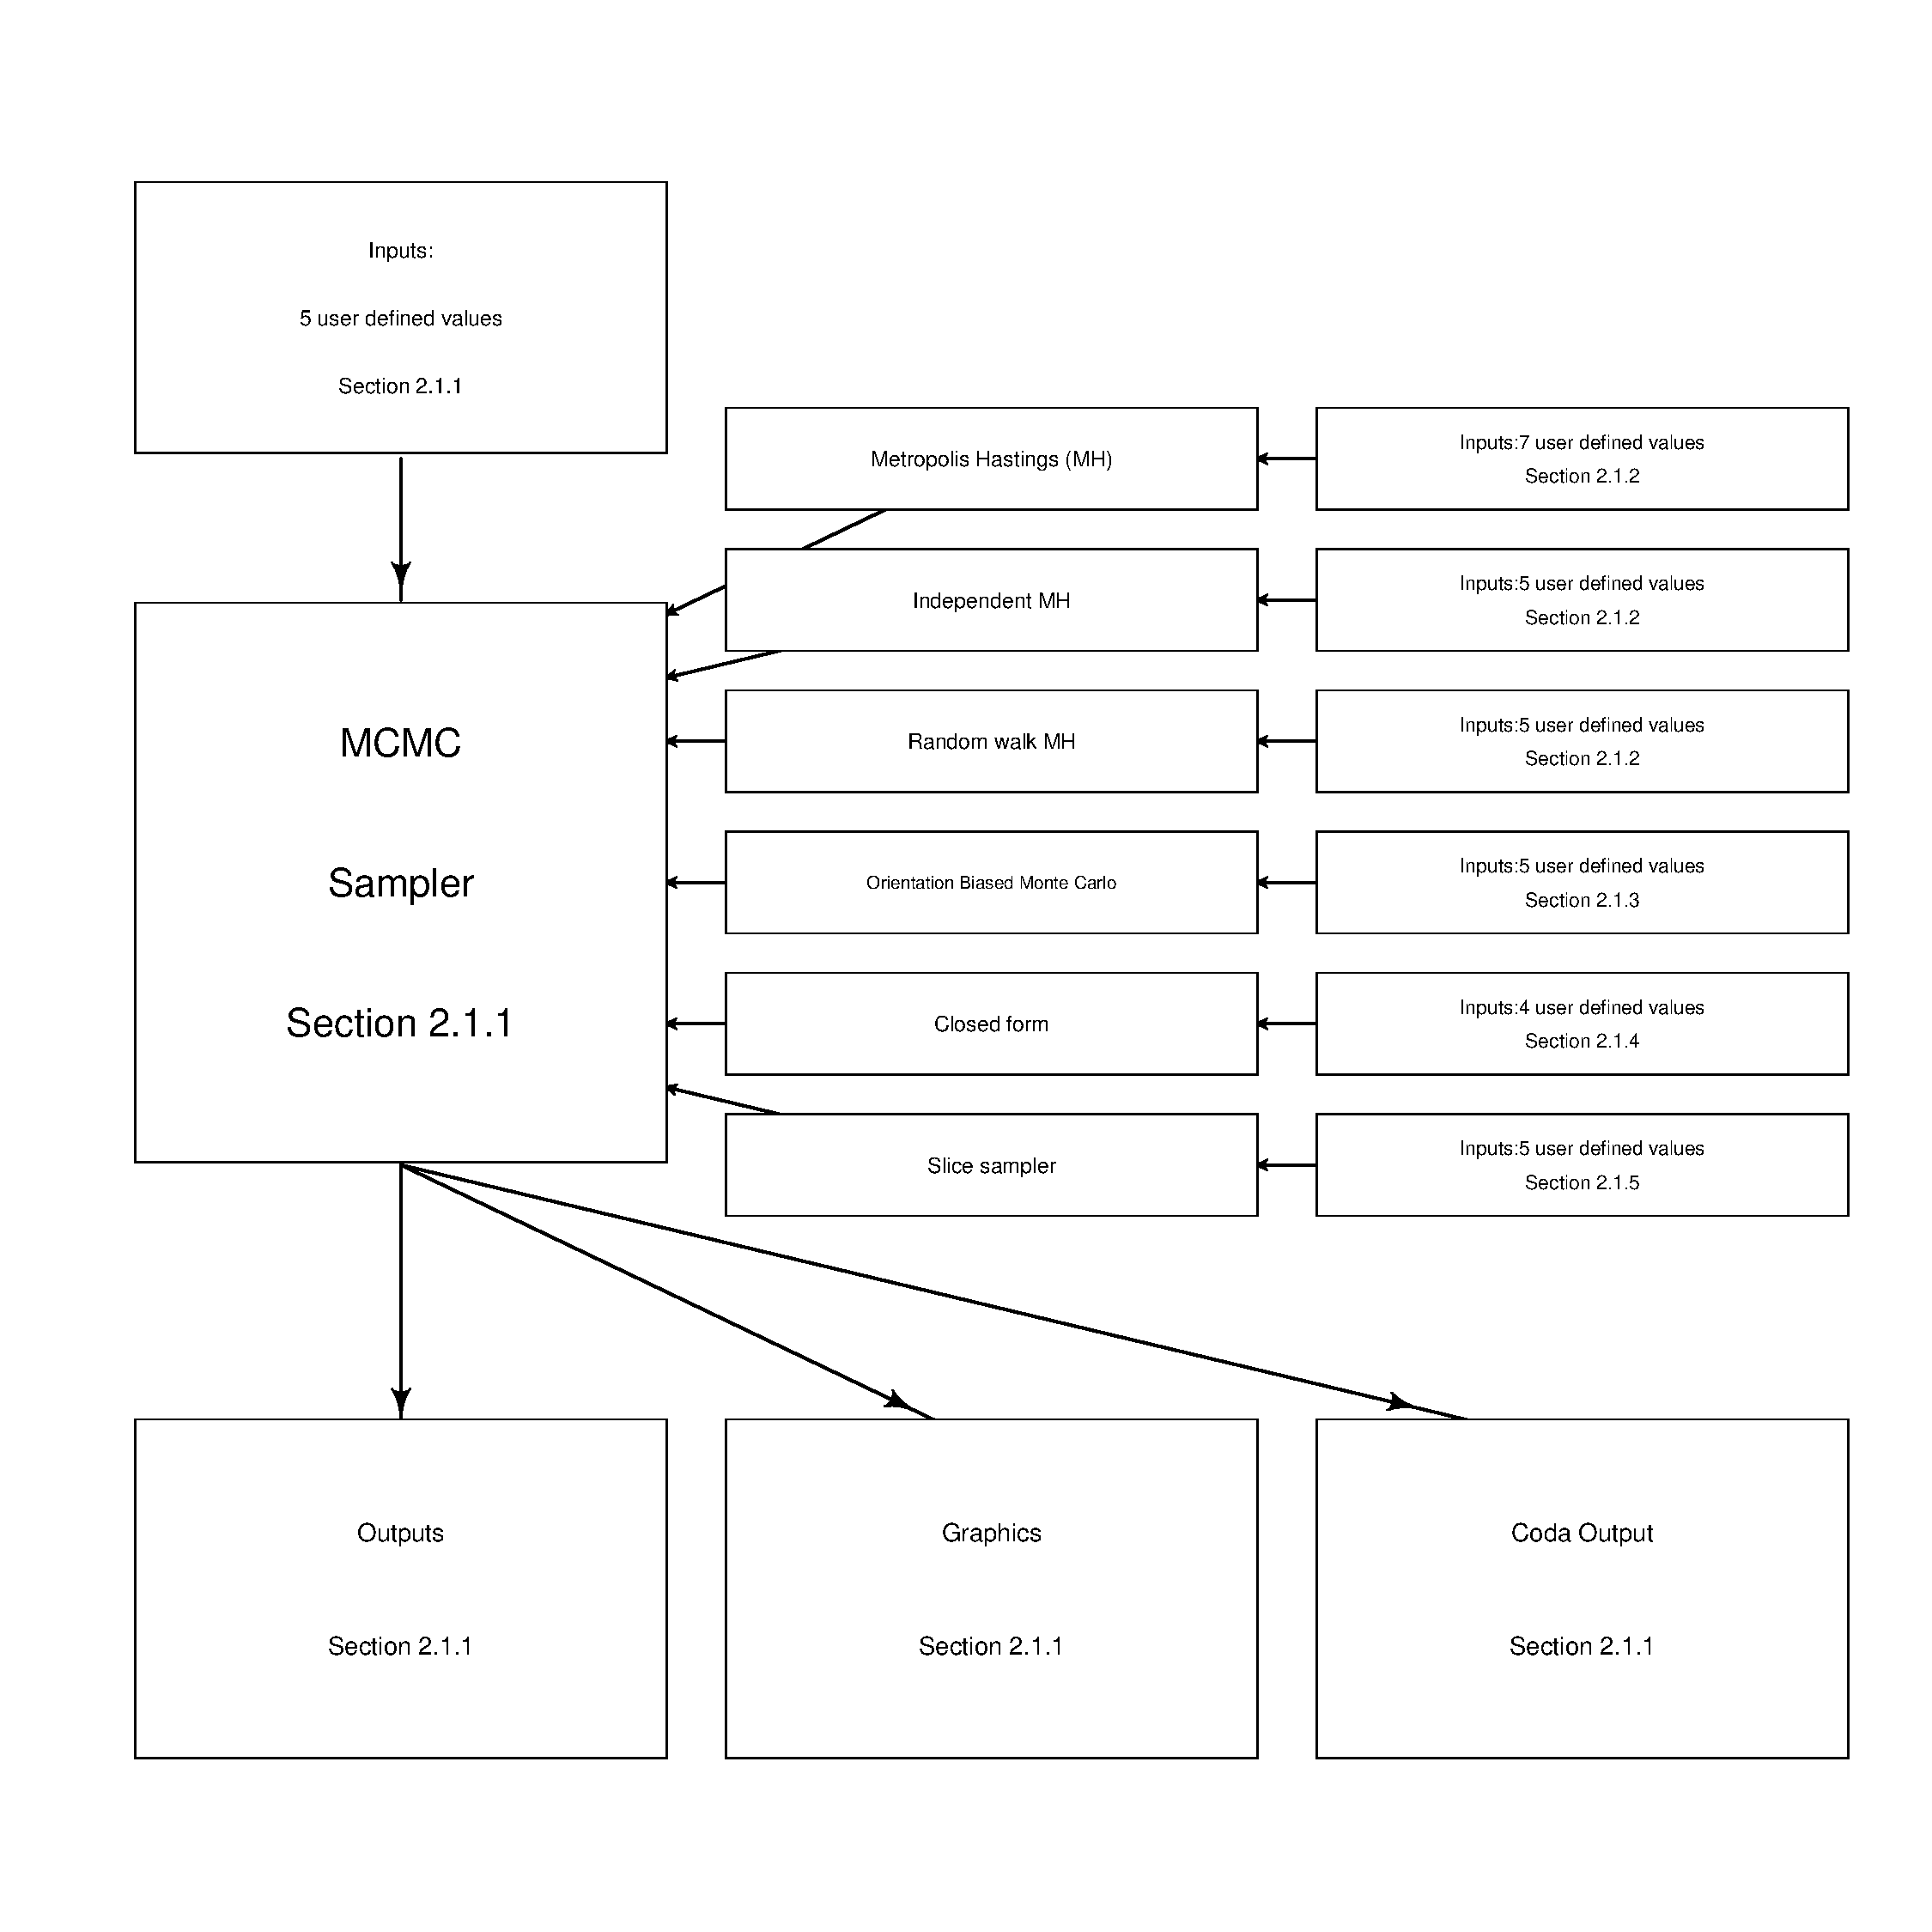
\includegraphics[width=18cm]{flowchart.pdf}    
  \end{center}
\caption{Flow chart illustrating the implementation of \pkg{PyMCMC}.\label{fig:Flow-chart-ofPyMCMC}}

\end{figure}


Figure \ref{fig:Flow-chart-ofPyMCMC} is a flow chart that depicts
the structure of \pkg{PyMCMC}. Essentially, the implementation of an MCMC
sampler can be seen to centred around the class \code{MCMC}, which
acts as a container for various algorithms that are used in sampling
from the conditional posterior distributions that make up the MCMC
sampling scheme. 

The structure of the paper is as follows. In Section \ref{sec:Bayesian-Analysis}
the algorithms contained in \pkg{PyMCMC} and the user interface are described.
This includes the Gibbs sampler, the Metropolis based algorithms and
the slice sampler. Section \ref{sec:Bayesian-Analysis} also contains
a description of the Bayesian regression module. Section \ref{sec:Empirical-Illustrations}
contains three empirical examples that demonstrate how to use \pkg{PyMCMC}.
The first example demonstrates how to use the regression module for
the Bayesian analysis of the linear model. In particular, the stochastic
search variable selection algorithm, see \citet{GeorgeMcCulloch1993}
and \citet{MarinRobert2007}, is used to select a set of `most likely
models'. The second example demonstrates how to use \pkg{PyMCMC} to analyse
the loglinear model and the third example demonstrates how to use
\pkg{PyMCMC} to analyse a linear model with first order autoregressive errors.
Section \ref{sec:Using-PyMCMC-efficiently} contains discussion on
the efficient implementation of the MCMC algorithms using \pkg{PyMCMC}.
Section \ref{sec:PyMCMC-interacting-with} describes how to use \pkg{PyMCMC}
interatively with \proglang{R} and Section \ref{sec:Conclusions} concludes.


\section{Bayesian analysis}
\label{sec:Bayesian-Analysis}

Bayesian analysis quantifies information about the unknown parameter
vector of interest, $\bm{\theta},$ for a given data set, $\bm{y},$
through the joint posterior probability density function (pdf),
$p(\bm{\theta}|\bm{y}),$ which is defined such that \begin{equation}
  p(\bm{\theta}|\bm{y})\propto p(\bm{y}|\bm{\theta})\times
  p(\bm{\theta}),\label{eq:joint post}\end{equation} where
$p(\bm{y}|\bm{\theta})$ denotes the pdf of $\bm{y}$ given
$\bm{\theta}$ and $p(\bm{\theta})$ is the prior pdf for $\bm{\theta}.$
The most common approach used for inference about $\bm{\theta}$ is
MCMC.


\subsection{Markov chain Monte Carlo Methods and implementation}

In the following subsections, a brief description of each algorithm
and the associated programming interface is included.


\subsubsection{Markov chain Monte Carlo sampling}

If we partition $\bm{\theta}$ into $s$ blocks, that is
$\bm{\bm{\theta}}=\left(\bm{\theta}_{1},\bm{\theta}_{2},\ldots,\bm{\theta}_{s}\right)^{T},$
then the $j^{th}$\ step for a generic MCMC sampling scheme is given
by:

%
\begin{algorithm}[H]
\begin{description}
\item [{\textmd{1.}}] Sample\textbf{\ }$\bm{\theta}_{1}^{j}$ from $p\left(\bm{\theta}_{1}|\bm{y,}\bm{\theta}_{2}^{j-1},\bm{\theta}_{3}^{j-1},\ldots,\bm{\theta}_{s}^{j-1}\right),$ 
\item [{\textmd{2.}}] Sample $\bm{\theta}_{2}^{j}$ from $p\left(\bm{\theta}_{2}|\bm{y,}\bm{\theta}_{1}^{j},\bm{\theta}_{3}^{j-1},\bm{\theta}_{4}^{j-1},\ldots,\bm{\theta}_{s}^{j-1}\right),$

\begin{description}
\item [{$\vdots$}]~
\end{description}
\item [{\textmd{s.}}] Sample $\bm{\theta}_{s}^{j}$ from $p\left(\bm{\theta}_{s}|\bm{y,}\bm{\theta}_{1}^{j},\bm{\theta}_{2}^{j},\ldots,\bm{\theta}_{s-1}^{j}\right).$ 
\end{description}
\caption{Gibbs sampler}
\label{alg:MCMC}
\end{algorithm}

An important special case of Algorithm \ref{alg:MCMC} is the Gibbs
sampler, which is an algorithm that is proposed in
\citet{GelfandSmith1990}. Specficially, when each of
$\bm{\theta}_{1},\bm{\theta}_{2},\dots,\bm{\theta}_{s},$ is sampled
from a closed form then this algorithm corresponds to that of the
Gibbs sampler. \pkg{PyMCMC} contains a class that facilitates the
implementation of Algorithm \ref{alg:MCMC}, in which the user must
define functions to sample from each block, ie. a function for each of
$\bm{\theta}_{i},$ for $i=1,\dots,s.$ These functions may be defined
using the Metropolis based or slice sampling algorithms that are part
of \pkg{PyMCMC}. The class is named \code{MCMC} and the following
arguments are required in the initialisation of the class:

\begin{description}
\item[\code{nit}:]  The number of iterations. 
\item[\code{burn}:]  The burn in length of the MCMC sampler. 
\item[\code{data}:] A dictionary (\proglang{Python} data structure)
  containing any data, functions or objects that the user would like
  to have access to when defining the functions that are called from
  the Gibbs sampler.
\item[\code{blocks}:] A list (\proglang{Python} data structure)
  containing functions that are used to sample from the full
  conditional posterior distributions of interest.
\item[\code{{*}{*}kwargs}] Optional arguments:
  
  \begin{description}
  \item[\code{loglike}] A tuple containing a function that evaluates
    the log-likelihood, number of parameters and the name of the
    dataset. For example: \code{loglike = (loglike, nparam, `yvec')}.
    If this is defined then the log-likelihood and the BIC will be
    reported in the standard output.
  \item[\code{transform}] A dictionary, where the keys are the names
    of the parameters and the associated values are functions that
    transform the iterates stored in the MCMC scheme. This can be
    useful when the MCMC algorithm is defined under a particular
    parametersation, but where it is desirable to report the results
    under a different parameterisation.
\end{description}
\end{description}
Several functions are included as a part of the class:
\begin{description}
\item \code{sampler()} - Used to run the MCMC sampler. 
\item \code{get\_mean\_cov(listname)} - Returns the posterior
  covariance matrix for the parameters named in \code{listname}, where
  \code{listname} is a list that contains the parameter names of
  interest.
\item \code{get\_parameter(name)} - Returns the iterates for the named
  parameter including burnin.
\item \code{get\_parameter\_exburn(name)} - Returns the iterates for
  the named parameter excluding the burnin.
\item \code{get\_mean\_var(name)} - Returns the estimate from the MCMC
  estimation for the posterior mean and variance for the parameter
  defined by \code{name}.
\item \code{set\_number\_decimals(num)} - Sets the number of decimal
  places for the output.
\item \code{output({*}{*}kwargs)} - Used to produce output from the
  MCMC algorithm.
\end{description}
  \begin{description}
  \item \code{{*}{*}kwargs} - Optional arguments that control the
    output.
    \begin{description}
    \item \code{parameters}: A dictionary, list or string specifying
      the parameters that are going to be presented.
      \begin{itemize}
      \item If a string is passed (eg: \code{parameters = `beta'}),
        all elements of that parameter are given.
      \item If a list, (eg: \code{parameters = {[}`alpha',
          `beta'{]})}, all elements of each parameter in the list are
        given.
      \item If a dictionary (eg: \code{parameters =
          \{`alpha':\{`range':range(5)\}\})}, then there is the
        possibility to add an additional argument 'range' that tells
        the output to only print a subset of the parameters. The above
        example will print information for \code{alpha{[}0{]},
          alpha{[}1{]},..., alpha{[}4{]}} only.
      \end{itemize}
    \item \code{custom} - A user defined function that produces custom
      output.
    \item \code{filename} - A filename to which the output is printed.
      By default output will be printed to stdout.
    \end{description}
   
  \item \code{plot(blockname, {*}{*}kwargs)} - Create summary plots of
    the MCMC sampler.  By default, a plot of the marginal posterior
    density, an ACF plot and a trace plot are produced for each
    parameter in the block. The plotting page is divided into a number
    of subfigures. By default, the number of columns are approximately
    equal to the square root of the total number of subfigures divided
    by the number of different plot types.
  \end{description}
  \begin{enumerate}
  \item \code{blockname} The name of the parameter, for which summary
    plots are to be generated.
  \item \code{{*}{*}kwargs} - An optional dictionary
    (\proglang{Python} data structure) containing information to
    control the summary plots.  The available keys are summarised
    below:

    \begin{enumerate}
    \item \code{elements}: A list of integers specifying the elements
      that will be plotted. For example, if the blockname is
      \code{`beta'} and
      $\bm{\beta}=(\beta_{0},\beta_{1}\ldots\beta_{n})$ then you may
      specify elements as \code{elements = {[}0,2,5{]}.}.
    \item \code{plottypes}: A list giving the type of plot for each
      parameter. By default the plots are \code{`density'},
      \code{`acf'} and \code{`trace'}. A single string is also
      acceptable.
    \item \code{filename}: A string providing the name of an output
      file for the plot.  As a plot of a block may be made up of a
      number of subfigures, the output name will be modified to give a
      separate filename for each subfigure. For example, if the
      filename is passed as \code{`plot.png'}, and there are multiple
      pages of output, it will produce the files \code{plot001.png},
      \code{plot002.png}, etc.  The type of file is determined by the
      extension of the filename, but the output format will also
      depend on the plotting backend being used.  If the filename does
      not have a suffix, a default format will be chosen based on the
      graphics backend. Most backends support png, pdf, ps, eps and
      svg (see the documentation for \pkg{Matplotlib} for further
      details http://matplotlib.sourceforge.net).

    \item \code{individual}: A Boolean option. If true, then each
      subplot will be done on an individual page.
    \item \code{rows}: Integer specifying the number of rows of
      subfigures on a plotting page.
    \item \code{cols}: Integer specifying the number of columns of
      subfigures on a plotting page.
    \end{enumerate}

  \item \code{CODAoutput({*}{*}kwargs)} - Output the results in a
    format suitable for reading in with the statistical package
    Convergence Diagnostic and Output Analysis (CODA). By default,
    there will be two files created, \code{coda.txt} and
    \code{coda.ind}.

    \begin{enumerate}
    \item \code{{*}{*}kwargs} - An optional dictionary controlling the
      CODA output.

      \begin{enumerate}
      \item \code{filename}: A string to provide an alternative
        filename for the output.  If the file has an extension this
        will form the basis for the data file and the index file will
        be named by replacing the extension with ind. If no extension
        is in the filename then two files will be created and named by
        adding the extensions .txt and .ind to the given filename.
      \item \code{parameters}: A string, a list or a dictionary that
        specify the items written to file. It can be a string such as
        \code{`alpha'} or it can be a list (eg
        \code{{[}`alpha',`beta'{]}}) or it can be a dictionary (eg
        \code{\{`alpha':\{`range':{[}0,1,5{]}\}\}}.  If you supply a
        dictionary the key is the parameter name. It is also
        permissible to have a range key with a range of elements. If
        the range isn't supplied it is assumed that the user wants all
        of the elements.
      \item \code{thin}: Integer specifying how to thin the output.
        For examples if \code{thin = 10}, then every tenth element
        will be written to the CODA output.
      \end{enumerate}
    \end{enumerate}
\end{enumerate}

\subsubsection{Metropolis Hastings}
\label{sub:Metropolis-Hastings}

A particularly useful algorithm that is often used as a part of MCMC
samplers is the MH algorithm (Algorithm \ref{alg:MH}); see for example
\citet{RobertCassela1999}. This algorithm is usually required when we
cannot easily sample directly from $p(\bm{\theta}|\bm{y}),$ however,
we have a candidate density
$q(\bm{\theta}|\bm{y})=q(\bm{\theta}|\bm{y},\bm{\theta}^{j-1})$, which
in practice is close to $p(\bm{\theta}|\bm{y}$), and is more readily
able to be sampled. The MH algorithm at the $j^{th}$ iteration for
$j=1,2,\dots,M$ is given by the following steps:

%
\begin{algorithm}[H]
\begin{enumerate}
\item Draw a candidate $\bm{\bm{\theta}}^{\ast}$ from the density $q\left(\bm{\bm{\theta}}|\bm{y},\bm{\theta}^{j-1}\right),$ 
\item Accept $\bm{\theta}^{j}=\bm{\theta}^{\ast}$ with probability equal
to $\min\left\{ 1,\frac{p\left(\bm{\theta}^{\ast}|\bm{y}\right)}{p\left(\bm{\theta}^{j-1}|\bm{y}\right)}/\frac{q\left(\bm{\theta}^{\ast}|\bm{y},\bm{\theta}^{j-1}\right)}{q\left(\bm{\theta}^{j-1}|\bm{y},\bm{\theta}^{*}\right)}\right\} ,$ 
\item Otherwise $\bm{\theta}^{j}=\bm{\theta}^{j-1}.$ 
\end{enumerate}
\caption{Metropolis Hastings}
\label{alg:MH}
\end{algorithm}


\pkg{PyMCMC} includes a class for the MH algorithm, which is called
\code{MH}.  To initialise the class the user needs to define:
\begin{enumerate}
\item \code{func} - User defined function that returns a sample for
  the parameter of interest.
\item \code{actualprob} - User defined function that returns the log
  probability of the parameters of interest evaluated using the target
  density.
\item \code{probcandprev} - User defined function that returns the log
  of $q\left(\bm{\theta}^{\ast}|\bm{y},\bm{\theta}^{j-1}\right).$
\item \code{probprevcand} - User defined function that returns the log
  of $q\left(\bm{\theta}^{j-1}|\bm{y},\bm{\theta}^{*}\right).$
\item \code{init\_theta} - Initial value for the parameters of
  interest.
\item \code{name} - The name of the parameter of interest.
\item \code{{*}{*}kwargs} - Optional arguments:

\begin{enumerate}
\item \code{store}
\begin{enumerate}  
\item \code{`all'} (default), stores every iterate for the parameter
  of interest. This is required for certain calculations.
\item \code{`none'}, does not store any of the iterates from the parameter of
  interest.
\end{enumerate}
\item \code{fixed\_parameter} - Is used if the user wants to fix the
  parameter value that is returned. This is used for testing MCMC
  sampling schemes.  This command will override any other
  functionality.
\end{enumerate}
\end{enumerate}
\paragraph{Independent Metropolis Hastings}

The independent MH algorithm is a special case of the MH algorithm
described in Section \ref{sub:Metropolis-Hastings}. Specifically, the
independent MH algorithm is applicable when we have a candidate
density
$q(\bm{\theta}|\bm{y})=q(\bm{\theta}|\bm{y},\bm{\theta}^{j-1})$.  The
independent MH algorithm at the $j^{th}$ iteration for
$j=1,2,\ldots,M$ is given by Algorithm \ref{alg:IMH}.

%
\begin{algorithm}[H]
\begin{enumerate}
\item Draw a candidate $\bm{\bm{\theta}}^{\ast}$ from the density $q\left(\bm{\bm{\theta}}|\bm{y}\right),$ 
\item Accept $\bm{\theta}^{j}=\bm{\theta}^{\ast}$ with probability equal
to $\min\left\{ 1,\frac{p\left(\bm{\theta}^{\ast}|\bm{y}\right)}{p\left(\bm{\theta}^{j-1}|\bm{y}\right)}/\frac{q\left(\bm{\theta}^{\ast}|\bm{y}\right)}{q\left(\bm{\theta}^{j-1}|\bm{y}\right)}\right\} ,$ 
\item Otherwise accept $\bm{\theta}^{j}=\bm{\theta}^{j-1}.$ 
\end{enumerate}
\caption{Independent MH algorithm}
\label{alg:IMH}
\end{algorithm}


\pkg{PyMCMC} contains a class for the independent MH algorithm, named
\code{IndMH}.  To initialise the class the user needs to define:
\begin{enumerate}
\item \code{func} - A user defined function that returns a sample for
  the parameter of interest.
\item \code{actualprob} - A user defined function that returns the log
  probability of the parameters of interest evaluated using the target
  density.
\item \code{candpqrob} - A user defined function that returns the log
  probability of the parameters of interest evaluated using the
  candidate density.
\item \code{init\_theta} - Initial value for the parameters of interest.
\item \code{name} - Name of the parameter of interest.
\item \code{{*}{*}kwargs}- Optional arguments:

\begin{enumerate}
\item \code{store}
  \begin{enumerate}
  \item \code{`all'} (default), stores every iterate for the parameter
    of interest. This is required for certain calculations.
  \item \code{`none'}, does not store any of the iterates from the parameter
    of interest.
  \end{enumerate}
\item \code{fixed\_parameter} - Is used if the user wants to fix the
    parameter value that is returned. This is used for testing MCMC
    sampling schemes.  This command will override any other
    functionality.
  \end{enumerate}
\end{enumerate}

\paragraph{Random Walk Metropolis Hastings \protect \protect \\
}

A useful and simple way to construct an MH candidate distribution is
via\begin{equation}
  \bm{\theta}^{\ast}=\bm{\theta}^{j-1}+\bm{\bm{\varepsilon}},\label{random
    walk candidate}\end{equation} where $\bm{\varepsilon}$ is a random
disturbance vector. If $\bm{\varepsilon}$ has a distribution that is
symmetric about zero then the MH algorithm has a specific form that is
referred to as the random walk\textbf{\ }MH algorithm. In this case,
note that the candidate density is both independent of $\bm{y}$ and,
due to symmetry, \textbf{\
}$q\left(\bm{\theta}^{\ast}|\bm{\theta}^{j-1}\right)=q\left(\bm{\theta}^{j-1}|\bm{\theta}^{\ast}\right)$.
The random walk MH algorithm at the $j^{th}$ iteration for
$j=1,2,\ldots,M$ is given\emph{\ }by Algorithm \ref{alg:rwmh}.

%
\begin{algorithm}[H]
  \begin{enumerate}
  \item Draw a candidate $\bm{\theta}^{\ast}$ from equation
    (\ref{random walk candidate}) where the random disturbance
    $\bm{\varepsilon}$ has a distribution symmetric about zero.
  \item Accept $\bm{\theta}^{j}=\bm{\theta}^{\ast}$ with probability
    equal to $\min\left\{
      1,\frac{p\left(\bm{\theta}^{\ast}|\bm{y}\right)}{p\left(\bm{\theta}^{j-1}|\bm{y}\right)}\right\}
    $,
  \item Otherwise accept $\bm{\theta}^{j}=\bm{\theta}^{j-1}.$
  \end{enumerate}
  \caption{Random Walk MH}
\label{alg:rwmh}
\end{algorithm}


A typical choice for the distribution of $\bm{\bm{\varepsilon}}$ is a
Normal distribution,\emph{\ }that is $\bm{\varepsilon\sim}i.i.d.$
$\bm{N}\left(0,\bm{\Omega}\right)\ $ where the covariance matrix
$\bm{\Omega}$ is viewed as a tuning parameter. \pkg{PyMCMC} includes a
class for the random walk MH algorithm, named \code{RWMH}. The class
\code{RWMH} is defined assuming $\bm{\varepsilon}$ follows a normal
distribution. Note that more general random walk MH algorithms could
be constructed using the MH class. To initialise the class the user
must specify:
\begin{enumerate}
\item \code{post} - A user defined function for the log of full
  conditional posterior distribution for the parameters of interest.
\item \code{csig} - Scale parameter for the random walk MH algorithm.
\item \code{init\_theta} - Initial value for the parameter of interest.
\item \code{name} - Name of the parameter of interest.
\item \code{**kwargs} - Optional arguments:

  \begin{enumerate}
  \item store
    \begin{enumerate}
    \item \code{`all'} (default), stores every iterate for the
      parameter of interest. This is required for certain
      calculations.
    \item \code{`none'}, does not store any of the iterates from the
      parameter of interest.
    \end{enumerate}
  \item \code{fixed\_parameter} - Is used if the user wants to fix the
    parameter value that is returned. This is used for testing MCMC
    sampling schemes.  This command will override any other
    functionality.
  \item \code{adaptive} - \code{`GYS'}, Then the adaptive random walk
    MH algorithm of \citet{GarthwaiteYanScisson2010} will be used to
    optimise $\bm{\Omega}.$
  \end{enumerate}
\end{enumerate}

\subsubsection{Orientational bias Monte Carlo}

The multiple try Metropolis \citep{LuiLiangWong2000} generalises the
MH algorithm to allow for multiple proposals. The OBMC algorithm is a
special case of the multiple try Metropolis that is applicable when he
candidate density is symmetric. The OBMC Algorithm at iteration $j$ is
as follows:

%
\begin{algorithm}[H]
\begin{enumerate}
\item Draw $L$ candidates $\bm{\theta}_{l}^{\ast},$ $l=1,2,\ldots,L$,
  independently from the densities
  $q\left(\bm{\theta}|\bm{y},\bm{\theta}^{j-1}\right)$, where
  $q\left(\bm{\theta}|\bm{y},\bm{\theta}^{j-1}\right)$ is a symmetric
  function.
\item Construct a \textit{probability mass function (pmf)} by
  assigning to each\emph{\ }$\bm{\theta}_{l}^{\ast},$ a probability
  proportional to $p\left(\bm{\theta}_{l}^{\ast}|\bm{y}\right).$
\item Select $\bm{\theta}^{\ast\ast}$ randomly from this discrete
  distribution.
\item Draw $L-1$ reference points $\bm{r}_{l},$
  $l=1,2,\ldots,L-1$,\textbf{\ }independently from
  $q\left(\bm{\theta}|\bm{y},\bm{\theta}^{\ast\ast}\right)$ and set
  $\bm{r}_{L}=\bm{\theta}^{j-1}.$
\item Accept $\bm{\theta}^{j}=\bm{\theta}^{\ast\ast}$ with probability
  equal to $\min\left\{
    1,\frac{\sum_{l=1}^{L}p\left(\bm{\theta}_{l}^{\ast}|\bm{y}\right)}{\sum_{l=1}^{L}p\left(\bm{r}_{l}|\bm{y}\right)}\right\}
  $,
\item Otherwise accept $\bm{\theta}^{j}=\bm{\theta}^{j-1}.$
\end{enumerate}
\caption{Orientational Bias Monte Carlo}
\label{alg:obmc}
\end{algorithm}


\pkg{PyMCMC} implements a special case of the OBMC algorithm, for
which the candidate density is multivariate normal, making it a
generalisation of the random walk MH algorithm. The class for the OBMC
algorithm is named \code{OBMC}. To initialise the class the user must
specify:
\begin{enumerate}
\item \code{post} - A user defined function for the log of full
  conditional posterior distribution for the parameters of interest.
\item \code{ntry} - Number of candidates, $L$.
\item \code{csig} - A scale parameter for the OBMC algorithm.
\item \code{init\_theta} - Initial value for the parameter of interest. 
\item \code{{*}{*}kwargs} - Optional arguments:

  \begin{enumerate}
  \item \code{store}
    \begin{enumerate}
    \item \code{`all'} (default), stores every iterate for the
      parameter of interest. This is required for certain
      calculations.
    \item \code{`none'}, does not store any of the iterates from the
      parameter of interest.
      \end{enumerate}
    \item \code{fixed\_parameter} - Is used if the user wants to fix
      the parameter value that is returned. This is used for testing
      MCMC sampling schemes.  This command will override any other
      functionality.
  \end{enumerate}
\end{enumerate}

\subsubsection{Closed form sampler}

A class is included so that the user can specify a function to sample
the parameters of interest when there is a closed form solution. The
name of the class is \code{CFsampler}. To initialise the class the
user must specify:
\begin{enumerate}
\item \code{func} - User defined function that samples from the
  posterior distribution of interest.
\item \code{init\_theta} - Initial value for the unknown parameter of
  interest.
\item \code{name} - The name of the parameter of interest.
\item \code{{*}{*}kwargs} - Optional parameters:

\begin{enumerate}
\item \code{store}
  \begin{enumerate}
  \item \code{`all'} (default), stores every iterate for the parameter
    of interest. This is required for certain calculations.
  \item `none', does not store any of the iterates from the parameter
    of interest.
  \end{enumerate}
\item \code{fixed\_parameter} - Is used if the user wants to fix the
  parameter value that is returned. This is used for testing MCMC
  sampling schemes.  This command will override any other
  functionality.
\end{enumerate}
\end{enumerate}

\subsubsection{Slice sampler}

The slice sampler is useful for drawing values from complex densities;
see \citet{Radford2003} for further details. The required distribution
must be proportional to one or a multiple of several other functions
of the variable of interest;

\[p(\theta)\propto f_{1}(\theta)f_{2}(\theta)\cdots f_{n}(\theta).\]

A set of values from the distribution is obtained by iteratively
sampling a new value, $\omega,$ from the vertical \emph{slice} between
0 and $f_{i}(\theta)$, then sampling a value for the parameter
$\theta$ from the horizontal \emph{slice} that consists of the set of
possible values of $\theta$, for which the previously sampled
$\omega\le p(\theta)$.  This leads to the slice sampler algorithm,
which can be defined at iteration $j$ using Algorithm
\ref{alg:slicesamp}.

%
\begin{algorithm}[H]
\begin{enumerate}
\item For $i=1,2,\dots,n$, draw $\omega_{i}\sim\mbox{Unif}[0,f_{i}(\theta^{j-1})]$. 
\item Sample $\theta^{j}\sim\mbox{Unif}[A]$ where $A=\left\{ \theta:f_{1}(\theta)\ge\omega_{1}\in f_{2}(\theta)\ge\omega_{2}\in\cdots\in f_{n}(\theta)\ge\omega_{n}\right\} $. 
\end{enumerate}
\caption{Slice sampler}
\label{alg:slicesamp}
\end{algorithm}


In cases where the density of interest is not unimodal, determining
the exact set $A$ is not necessarily straightforward. The
\emph{stepping out} algorithm of \citet{Radford2003} is used to obtain
the set $A$.  This algorithm is applied to each of the $n$ slices to
obtain the joint maximum and minimum of the slice. This results in a
sampling interval that is designed to draw a new $\theta^{j}$ in the
neighbourhood of $\theta^{j-1}$ and may include values outside the
permissible range of $A$. The user is required to define an estimated
typical slice size ($ss$), which is the width of set $A$, along with
an integer value ($N$), which limits the width of any slice to $N\times ss$.
The stepping out algorithm (\ref{alg:steppingout}) is:

%
\begin{algorithm}[H]
\begin{enumerate}
\item Initiate lower (LB) and upper (UB) bounds for slice defined by set
$A$.\end{enumerate}
\begin{itemize}
\item $U\sim\mbox{Unif}(0,1)$; 

\begin{itemize}
\item $LB=\theta^{j-1}-ss{\times}U$, 
\item $UB=LB+ss$. 
\end{itemize}
\end{itemize}
\begin{enumerate}
\item Sample $V\sim\mbox{Unif}(0,1)$. 
\item Set $J=\mbox{Floor}(N{\times}V)$. 
\item Set $Z=(N-1)-J$. 
\item Repeat while $J>0$ and $\omega_{i}<f_{i}(LB)\forall i$;

\begin{itemize}
\item LB = LB - $ss$, 
\item $J=J-1$. 
\end{itemize}
\item Repeat while $Z>0$ and $\omega_{i}<f_{i}(UB)\forall i$;

\begin{itemize}
\item UB = UB + ss, 
\item Z = Z - 1. 
\end{itemize}
\item Sample $\theta^{j}\sim\mbox{Unif}(LB,UB)$. 
\end{enumerate}
\caption{Stepping out}
\label{alg:steppingout}
\end{algorithm}


The value of $\theta^{j}$ is accepted if it is drawn from a range
$(LB,UB)\in A$. If it is outside the allowable range due to the
interval $(LB,UB)$ being larger in range then the set $A$ we then
invoke a shrinkage technique to resample $\theta^{j}$ and improve the
sampling efficiency of future draws, until an acceptable $\theta^{j}$
is drawn.  The shrinkage algorithm is implemented as follows,
repeating this algorithm until exit conditions are met.

%
\begin{algorithm}[H]
\begin{enumerate}
\item $U\sim\mbox{Unif}(0,1)$. 
\item $\theta^{j}=LB+U{\times}(UB-LB)$;

\begin{itemize}
\item If $\omega_{i}<f_{i}(\omega_{i})\forall i$, accept $\theta^{j}$
and exit, 
\item Else if $\theta^{j}<\theta^{j-1}$, set $LB=\theta^{j}$ and return
to step 1, 
\item Else set $UB=\theta^{j}$ and return to step 1. 
\end{itemize}
\end{enumerate}
\caption{Shrinkage}
\label{alg:shrinkage}
\end{algorithm}


\pkg{PyMCMC} includes a class for the slice sampler named
\code{SliceSampler.  }To initialise the class the user must define:
\begin{enumerate}
\item \code{func} - A $k$ dimensional list containing the set of log
  functions.
\item \code{init\_theta} - An initial value for $\theta$.
\item \code{ssize} - A user defined value for the typical slice size.
\item \code{sN} - An integer limiting slice size to $N\times ss$.
\item \code{{*}{*}kwargs} - Optional arguments:
   
  \begin{enumerate}
  \item \code{store}
    \begin{enumerate}
    \item \code{`all'} (default), stores every iterate for the
      parameter of interest. This is required for certain
      calculations.
    \item `none', does not store any of the iterates from the
      parameter of interest.
    \end{enumerate}
  \item fixed\_parameter - Is used if the user wants to fix the
    parameter value that is returned. This is used for testing MCMC
    sampling schemes.  This command will override any other
    functionality.
  \end{enumerate}
\end{enumerate}

\subsection{Normal linear Bayesian regression model}
\label{sec: Regression Model}

Many interesting models are partly linear for a subset of the unknown
parameters. As such drawing from the full conditional posterior
distribution for the associated parameters may be equivalent to
sampling the unknown parameters in a standard linear regression model.
\pkg{PyMCMC} includes several classes that aid in the analysis of
linear or partly linear models. In particular the classes
\code{BayesRegression}, \code{CondRegBetaSampler},
\code{CondScaleSampler} and \code{StochasticSearch} are useful for
this purpose. These classes are described in this section.  For the
standard linear regression model (see \cite{Zellner1971}), assume the
$\left(n\times1\right)$ observational vector, $\bm{y},$ is generated
according to\begin{equation}
  \bm{y}=\bm{X}\bm{\beta}+\bm{\varepsilon};\,\,\,\bm{\varepsilon}\sim
  N(\bm{0},\sigma^{2}\bm{I}),\label{eq:regression}
\end{equation} where
$\bm{X}$ is an $(n\times k)$ matrix of regressors, $\bm{\beta}$ is a
$\left(k\times1\right)$ vector of regression coefficients and
$\bm{\varepsilon}$ is a normally distributed random variable with a
mean vector $\bm{0}$ and an $\left(n\times n\right)$ covariance
matrix, $\sigma^{2}\bm{I}.$ Assuming that both $\bm{\beta}$ and
$\sigma$ are unknown then the posterior distribution for
(\ref{eq:regression}) is given by\begin{equation}
  p(\bm{\beta},\sigma|\bm{y},\bm{X})\propto
  p(\bm{y}|\bm{X},\bm{\beta},\sigma)\times
  p(\bm{\beta},\sigma),\label{eq:post regression}
\end{equation} where
\begin{equation}
  p(\bm{y}|\bm{X},\bm{\beta},\sigma)\propto\sigma^{-n}\exp\left\{
    -\frac{1}{2\sigma^{2}}\left(\bm{y}-\bm{X}\bm{\beta}\right)^{T}\left(\bm{y}-\bm{X}\bm{\beta}\right)\right\}
  ,\label{eq:likelihood regression}
\end{equation} is the joint
\emph{pdf} for $\bm{y}$ given $\bm{X}$, $\bm{\beta}$ and
$\sigma$, and\emph{ $p(\bm{\beta},\sigma)$ } denotes the joint
prior \emph{pdf} for $\bm{\beta}$ and $\sigma$.

A class named \code{BayesRegression} is defined to sample from the
posterior distribution in (\ref{eq:post regression}). One of four
alternative priors may be used in the specification of the model.  The
default choice is Jeffreys prior. Denoting the full set of unknown
parameters as $\bm{\theta}=(\bm{\beta}^{T},\sigma)^{T},$ then Jeffreys
prior is defined such that 
\begin{equation}
  p(\bm{\theta})\propto|I(\bm{\theta})|^{-1/2},\label{eq:Jeffrey's
    Prior}
\end{equation} 
where $I(\bm{\theta})$ is the Fisher information matrix for
$\bm{\theta}.$ For the normal linear regression model in
\ref{eq:regression}, given the assumption that $\beta$ and $\sigma$
are \emph{a priori} independent, Jeffreys prior is flat prior over the
real number line for $\beta$, and for $\sigma$ is distributed such
that
\begin{equation}
		p\left(\sigma\right)\propto\frac{1}{\sigma}.
\end{equation}
See \cite{Zellner1971} for further details on Jeffreys prior. Three
alternative informative prior specifications are allowed, namely the
normal-gamma, the normal-inverted-gamma and Zellner's g-prior; see
\cite{Zellner1971} and \cite{MarinRobert2007} for further details.
The normal-gamma prior is specified such that
\begin{equation}
  \bm{\beta}|\kappa\sim
  N(\bm{\underline{\beta}},\underline{\bm{V}}^{-1}),\,\,\,\kappa\sim
  G\left(\frac{\underline{\nu}}{2},\frac{\underline{S}}{2}\right),\label{eq:Normal
    Gamma}
\end{equation} 
where $\kappa=\sigma^{-2}$ and $\underline{\beta,}$
$\underline{\bm{V}},$ $\underline{\nu}$ and $\underline{S}$ are prior
hyperparameters that take user defined values. For the Normal-gamma
prior, \code{BayesRegression} produces estimates for\emph{
  $\left(\kappa,\bm{\beta}^{T}\right)^{T}$ }rather than
$\left(\sigma,\bm{\beta}^{T}\right)$ . The Normal-inverted gamma prior
is specified such that
\begin{equation}
  \bm{\beta}|\sigma^{-2}\sim`
  N(\bm{\underline{\beta}},\underline{\bm{V}}^{-1}),\,\,\,\sigma^{-2}\sim
  IG\left(\frac{\underline{\nu}}{2},\frac{\underline{S}}{2}\right),\label{eq:Normal
    Inverted Gamma}
\end{equation} 
where $\underline{\beta,}$ $\underline{\bm{V}},$ $\underline{\nu}$ and
$\underline{S}$ are prior hyperparameters, which take values that are
set by the user. Zellner's g-prior is specified such that
\begin{equation} \bm{\beta}|\sigma\sim
  N\left(\underline{\bm{\beta}},g\sigma^{2}\left(X^{T}X\right)^{-1}\right),\,\,\,
  p(\sigma)\propto\sigma^{-1},\label{eq:g-prior}
\end{equation}
where $\bm{\underline{\beta}}$ and $g$ are hyperparameters with values
that are specified by the user. To initialise the class
\code{BayesRegression} the user must specify:
\begin{enumerate}
\item \code{yvec} - One dimensional \pkg{Numpy} array containing the
  data.
\item \code{xmat} - Two dimensional \pkg{Numpy} array contain the
  regressors.
\item \code{{*}{*}kwargs} - Optional arguments:

  \begin{enumerate}
  \item \code{prior} - A list contain the name of the prior and the
    corresponding hyperparameters. Examples: \code{prior =
      {[}`normal\_gamma', betaubar, Vubar, nuubar, Subar{]}},
    \code{prior = {[}`normal\_inverted\_gamma',betaubar, Vubar,
      nuubar, Subar{]}} and \code{prior = {[}`g\_prior', betaubar,
      g{]}}. If none of these options are chosen or they are
    miss-specified then the default prior will be Jeffreys prior.
  \end{enumerate}
\end{enumerate}
\code{BayesRegression} contains several functions that may be of
interest to the user. In particular:
\begin{enumerate}
\item \code{sample()} - Returns a sample of $\sigma$ and $\bm{\beta}$
  from the joint posterior distribution for the normal-inverted gamma
  prior, Jeffreys prior and Zellner's g-prior. If the normal-gamma
  prior is specified then \code{sample()} returns $\kappa$ and
  $\bm{\beta}.$
\item \code{update\_yvec(yvec)} - Updates yvec in
  \code{BayesRegression}. This is often useful when the class is being
  used as a part of the MCMC sampling scheme.
\item \code{update\_xmat(xmat)} - Updates xmat in
  \code{BayesRegression}. This is often useful when the class is being
  used as a part of the MCMC sampling scheme.
\item \code{loglike(scale, beta)} - Returns the log-likelihood.
\item \code{posterior\_mean()} - Returns the posterior mean for the
  scale parameter (either $\sigma$ or $\kappa$ depending on the
  specified prior) and $\bm{\beta}.$
\item \code{get\_posterior\_covmat()} - Returns the posterior
  covariance matrix for $\bm{\beta}$.
\item \code{bic()} - Returns the Bayesian information criterion; see
  \cite{KassRaftery1995} for details.
\item \code{plot({*}{*}kwargs)} - Produces standard plots.
  Specifically the marginal posterior density intervals for each
  element of $\bm{\beta}$ and for the scale parameter ($\sigma$ or
  $\kappa)$.
\item \code{residuals} - Returns the residual vector from the
  regression analysis.  The residuals are calculated with $\bm{\beta}$
  evaluated at the marginal posterior mean.
\item \code{output} - Produces standard output for the regression
  analysis.  This includes the means, standard deviations and HPD
  intervals for the marginal posterior densities for each element of
  $\bm{\beta}$ and for the scale parameter ($\sigma$ or $\kappa)$. The
  output also reports the log-likelihood and the Bayesian information
  criterion (BIC).
\end{enumerate}
In MCMC sampling schemes it is common that for a subset of the unknown
parameters of interest the full conditional posterior distribution
will correspond to that of a linear regression model, where the scale
parameter is known. For the linear regression model specified in
(\ref{eq:regression}) the posterior distribution for the case that
$\sigma$ is known is as follows
\begin{equation} 
p\left(\bm{\beta}|\bm{y},\bm{X},\bm{\beta},\sigma\right)\propto
  p(\bm{y}|\bm{X},\bm{\beta},\sigma)\times
  p(\bm{\beta}),\label{eq:post_condbeta}
\end{equation} where
$p(\bm{y}|\bm{X},\bm{\beta},\sigma)$ is described in
(\ref{eq:likelihood regression}) and $p(\bm{\beta})$ is the prior
\emph{pdf} for $\bm{\beta}.$ To sample from (\ref{eq:post_condbeta}) a
class named \code{CondBetaRegSampler} can be used. The user may
specify one of three alternative priors.  The default prior is
Jeffreys prior, which for $\bm{\beta}$ is simply a flat prior over
the real number line. A normally distributed prior for $\bm{\beta}$ is
another option, and can be specified such that\[ \bm{\beta}\sim
N\left(\underline{\beta},\bm{V}^{-1}\right).\] The user may also
specify their \emph{a priori} beliefs using Zellner's g-prior, where\[
\bm{\beta}|\sigma\sim
N\left(\bm{\beta},g\sigma^{2}\bm{X}^{T}\bm{X}\right).\] To initialise
the class the user must specify:
\begin{enumerate}
\item \code{yvec} - A one dimensional \pkg{Numpy} array containing the
  data.
\item \code{xmat} - A two dimensional \pkg{Numpy} array containing the
  regressors.
\item \code{{*}{*}kwargs} - Optional arguments:

\begin{enumerate}
\item \code{prior} - A list containing the name of the prior and the
  corresponding hyperparameters. Examples: \code{prior={[}`normal',
    betaubar, Vubar{]} or {[}`g\_prior', betaubar, g{]}}. If none of
  these options are chosen or they are miss-specified then the default
  prior will be Jeffreys prior.
\end{enumerate}
\end{enumerate}
\code{CondBetaRegSampler} contains several functions that may be of
interest to the user. In particular:

\begin{enumerate}

\item \code{sample(sigma)} - Returns a sample of $\bm{\beta}$ from the
  posterior distribution specified in \ref{eq:post_condbeta}.
\item \code{get\_marginal\_posterior\_mean()} - Returns the marginal
  posterior mean for \ref{eq:post_condbeta}.
\item \code{get\_marginal\_posterior\_precision()} - Returns the
  marginal posterior precision for the linear conditional posterior
  distribution specified in \ref{eq:post_condbeta}.
\item \code{update\_yvec(yvec)} - Updates yvec in
  \code{CondBetaRegSampler}. This is often useful when the class is
  being used as a part of an MCMC sampling scheme.
\item \code{update\_xmat(xmat)} - Updates xmat in
  \code{CondBetaRegSampler}. This is often useful when the class is
  being used as a part of an MCMC sampling scheme.
\end{enumerate}
Many Bayesian models contain linear components with unknown scale
parameters, hence a class has been specified named
\code{CondScaleSampler}, which can be used to individually sample
scale parameters from their posterior distributions. In particular, we
wish to sample from
\begin{equation} p(\sigma|\bm{y},\bm{\theta}),\label{eq:posterior
    sigma}
\end{equation} where $\bm{\theta}$ is the set of unknown
parameters of interest excluding $\sigma.$ The user may choose to use
one of three priors.  The Jeffreys prior, which for $\sigma$ given
the posterior in (\ref{eq:posterior sigma}) is as follows \[
p(\sigma)\propto\frac{1}{\sigma}.\] The second option is to specify an
inverted-gamma prior, such that\[ \sigma\sim
IG\left(\frac{\underline{\nu}}{2},\frac{\underline{S}}{2}\right).\]
Alternatively, the user may specify a gamma prior for
$\kappa=\frac{1}{\sigma^{2}},$ where\[ \kappa\sim
G\left(\frac{\underline{\nu}}{2},\frac{\underline{S}}{2}\right).\] To
initialise the class \code{CondScaleSamper} the user may first
specify:
\begin{enumerate}
\item \code{{*}{*}kwargs} - Options arguments:
\begin{enumerate}
\item \code{prior} - List containing the name of the prior and the
  corresponding hyperparameters. Examples:
  \code{prior={[}`gamma',nuubar,subar{]}} or
  \code{{[}`inverted-gamma', nuubar, subar{]}}. If no prior is
  specified the Jeffreys prior is used.
\end{enumerate}
\end{enumerate}
\pkg{PyMCMC} also includes another class that can be used for the
direct analysis of the linear regression model. The class is called
\code{StochasticSearch} and can be used in conjunction with the class
\code{MCMC}, for the purpose of variable selection.

The stochastic search algorithm can be used for variable selection in
the linear regression model. Given a set of $k$ possible regressors
there are $2^{k}$ models to choose from. The stochastic search
algorithm, as proposed by \citet{GeorgeMcCulloch1993}, uses the Gibbs
sampler to select a set of `most likely' models. The stochastic search
algorithm is implemented in the class \code{StochasticSearch}. The
specific implementation follows \citet{MarinRobert2007}. The algorithm
introduces the vector $\bm{\gamma},$ which is used to select the
explanatory variables that are to be included in the model. In
particular, $\bm{\gamma}$ is defined to be a binary vector of order
$k$, whereby the inclusion of the $i^{th}$regressor implies that the
$i^{th}$element of $\bm{\gamma}$ is a one, whilst the exclusion of the
$i^{th}$ regressor implies that the $i^{th}$ element is zero.  It is
assumed that the first element of the design matrix is always included
and should typically be a column of ones which is used to represent
the constant or intercept in the regression. The algorithm specified
to sample $\bm{\gamma}$ is a single move Gibbs sampling scheme; for
further details see \citet{MarinRobert2007}.

To use the class \code{StochasticSearch }the user must specify their
\emph{a priori} beliefs that the unknown parameters of interest,
$(\sigma,\bm{\beta}^{T})^{T},$ are specified according Zellner's
g-prior, which is described in (\ref{eq:g-prior}).
\emph{StochasticSearch }is designed to be used in conjunction with the
MCMC sampling class. To initialise \code{StochasticSearch} the user
must specify:
\begin{enumerate}
\item \code{yvec} - One dimensional \pkg{Numpy} array containing the
  dependent variable.
\item \code{xmat} - Two dimensional \pkg{Numpy} array containing the
  regressors.
\item \code{prior} - List with the following structure
  \code{{[}betaubar, g{]}}.
\end{enumerate}
The class \code{StochasticSearch} also contains the following
function:
\begin{enumerate}
\item \code{sample\_gamma(store)} - Returns a sample of $\bm{\gamma}.$
  The only argument to pass into the function \code{sample\_gamma} is
  the storage dictionary that is passed by default to each of the
  classes that are called from the class \code{MCMC }in \pkg{PyMCMC}.
\end{enumerate}

\section{Empirical illustrations}
\label{sec:Empirical-Illustrations}

\pkg{PyMCMC} is illustrated though three examples. Specifically, a
linear regression example with variable selection, a log-linear
example and a linear regression model with first order autoregressive
errors.  For each example, the model of interest is specified, then
the code used for estimation is shown, following which a brief
description of code is given. Each example uses the module for
\pkg{PyMCMC}, along with the \proglang{Python} libraries \pkg{Numpy},
\pkg{Scipy} and \pkg{Matplotlib}: see \citet{NumpyScipy, Matplotlib}
for further details of these Python libraries.  Example 3 further uses
the library \pkg{Pysparse}.


\subsection{Example 1: Linear regression model: Variable selection and
  estimation}

The normal linear regression model in (\ref{eq:regression}) is used
for the analysis.  The data set of interest contains 19 regressors. To
select the set of `most probable' regressors we can use the stochastic
search variable selection approach described in Section \ref{sec:
  Regression Model}.

\subsubsection{Example code: Variable selection in regression}


\begin{lstlisting}[basicstyle={\scriptsize},numbers=left]
import os
from numpy import loadtxt, hstack, ones, random, zeros, asfortranarray, log
from pymcmc.mcmc import MCMC, CFsampler
from pymcmc.regtools import StochasticSearch, BayesRegression
import pymcmc

datadir = os.path.join(os.path.dirname(pymcmc.__file__),'data')

def samplegamma(store):
    return store['SS'].sample_gamma(store)

random.seed(12346)

data = loadtxt(os.path.join(datadir,'yld2.txt'))
yvec = data[:, 0]
xmat = data[:, 1:20]
xmat = hstack([ones((xmat.shape[0], 1)), xmat])

data ={'yvec':yvec, 'xmat':xmat}
prior = ['g_prior', zeros(xmat.shape[1]), 100.]
SSVS = StochasticSearch(yvec, xmat, prior);
data['SS'] = SSVS

initgamma = zeros(xmat.shape[1], dtype ='i')
initgamma[0] = 1
simgam = CFsampler(samplegamma, initgamma, 'gamma', store ='none')

ms = MCMC(20000, 5000, data, [simgam])
ms.sampler()
ms.output(filename ='vs.txt')
ms.output(custom = SSVS.output, filename = 'SSVS.out')
ms.output(custom = SSVS.output)

txmat = SSVS.extract_regressors(0)
g_prior = ['g_prior', 0.0, 100.]
breg = BayesRegression(yvec,txmat,prior = g_prior)
breg.output(filename = 'SSVS1.out')
breg.plot()
\end{lstlisting}


The code is organised so that the user defined functions are at the
top and the main program is at the bottom.  Essentially the user
defined functions that are called from the class \code{MCMC}, for
which there is one in this case, all take the argument \code{store},
which is a dictionary (\proglang{Python} data structure) that is
passed to all functions that are called from the MCMC sampler.  The
purpose of \code{store} is that it contains all the data required to
define functions that sample from, or are used in the evaluation of,
the posterior distribution. For example, in line 15,
\code{store{[}`SS'{]}} contains the class instance for
\code{StochasticSearch}.  Essentially, any information that is stored
in the dictionary \code{data}, which is defined on line 30 and
augmented to include the class instance for \code{StochasticSearch}
defined on line 31 can be accessed from the dictionary \code{store}.
Note that the dictionary \code{data} is an argument that is used in
the initialisation of the \code{MCMC} class on line 39. In addition to
the information stored in \code{data,} the value of the previous
iterate for each block of the Gibbs scheme is also a component of the
dictionary store. For example on line 36 the class instance
\code{simgam} is initialised. Note that the name \code{`gamma'} is
specified to refer to the parameter $\bm{\gamma}.$ If the user wanted
to access the current iteration for \code{`gamma'} from any of the
functions called from \code{MCMC}, this would simply be done using
\code{store{[}`gamma'{]}}.  This feature is not used in this example,
but can be seen in the proceding examples. A brief description of the
code is as follows:
\begin{itemize}
\item Lines 1-5 import the classes and functions that are required in
  this example.
\item Line 7 is used to obtain the path of the data if installed
  using setup.py. Note that this step will not be necessary for normal
  usage of \pkg{PyMCMC}.
\item Lines 9-10 define the function that is used to sample
  $\bm{\gamma}.$
\item The main program starts at line 12 with the command to set the random seed.
\item Lines 14-17 are used to load the data, from which arrays
  $\bm{y}$ (\code{yvec}) and $\bm{X}$ (\code{xmat}) are constructed.
\item Lines 19-22 construct the dictionary \code{data}, which includes
  \code{yvec, xmat} and the class instance of \code{StochasticSearch}.
\item Line 26 defines the class instance \code{simgam}, which defines
  the block of the MCMC scheme to sample $\bm{\gamma}$.
\item Line 28 defines the class instance of \code{MCMC}. Note that the
  Gibbs sampler will run for 20000 iterations, of which the first 5000
  iterations will constitute the burnin and be discarded for the
  calculations in the output. The Gibbs sampler contains one block,
  which is defined by the class instance \code{simgam}.
\item Line 29 runs the MCMC sampler.
\item Line 30 produces the standard output for the MCMC sampler, which
  is saved in the file \code{`vs.txt'}.
\item Line 31 produces the custom output from the stochastic search
  class and is sqaved in the file \code{'SSVS.out'}.
\item Line 32 proqduces the custom output for the stochastic search
  class and writes it to the screen.
\item Lines 34-37 produces regression output, from a Bayesian
  regression analysis based on the most probable model.
\item Line 38 produces standard plots from the Bayesian regression
  analysis.
\end{itemize}

\subsubsection{Analysis}

The data used in this example are a response of crop yield modelled
using various chemical measurements from the soil. As the results of
the chemical analysis of soil cores are done in a laboratory, many
input variables are available (30) and the data analyst would like to
determine the variables that are most appropriate to use in the model.

%
\begin{minipage}[t]{1\columnwidth}%
\begin{verbatim}

Most likely models ordered by decreasing posterior probability

------------------------------------------------------------
probability | model       
------------------------------------------------------------
0.09353333  | 0,12        
0.0504      | 0,11,12     
0.026       | 0,10,12     
0.01373333  | 0,9,12      
0.01353333  | 0,8,12      
0.013       | 0,4,12      
0.01293333  | 0,12,19     
0.01206667  | 0,7,12      
0.01086667  | 0,11,12,17  
0.01086667  | 0,12,17     
------------------------------------------------------------

\end{verbatim}%
\end{minipage}

As indicated earlier, the MCMC analysis is conducted using 20000
iterations, of which the first 5000 are discarded. The estimation
takes 10.35 seconds in total.  The results indicate that a model
containing variable 12 along with a constant (indicated in the table
by 0) is the most likely (prob = 0.09). Furthermore, variable 12 is
contained in each of the 10 most likely models, indicating its strong
association with crop yield.

%
\begin{minipage}[t]{1\columnwidth}%
\begin{verbatim}

          ---------------------------------------------------           
                   Bayesian Linear Regression Summary                   
                                g_prior                                 
          ---------------------------------------------------           
                    mean          sd         2.5%       97.5%
     beta[0]     -0.1254      0.1058      -0.3361     0.08533
     beta[1]      0.7587      0.0225       0.7139      0.8035
       sigma      0.3853     0.03152          NA         NA

loglikelihood = -4.143      
marginal likelihood = nan         
BIC  = -0.4017     

\end{verbatim}%
\end{minipage}

The parameter associated with variable 12, $\hat{\beta_{1}}$, is
estimated as a positive value, 0.7587, with a 95\% credible interval
{[}0.7139,~0.8035{]}. We note that zero is not contained in the
credible interval, hence the crop yield increases with higher values
of variable 12. The marginal posterior densities (Figure \ref{Flo:mpd
  reg}) illustrate that this effect is far from zero. %

\begin{figure}[t!]
  \begin{center}
    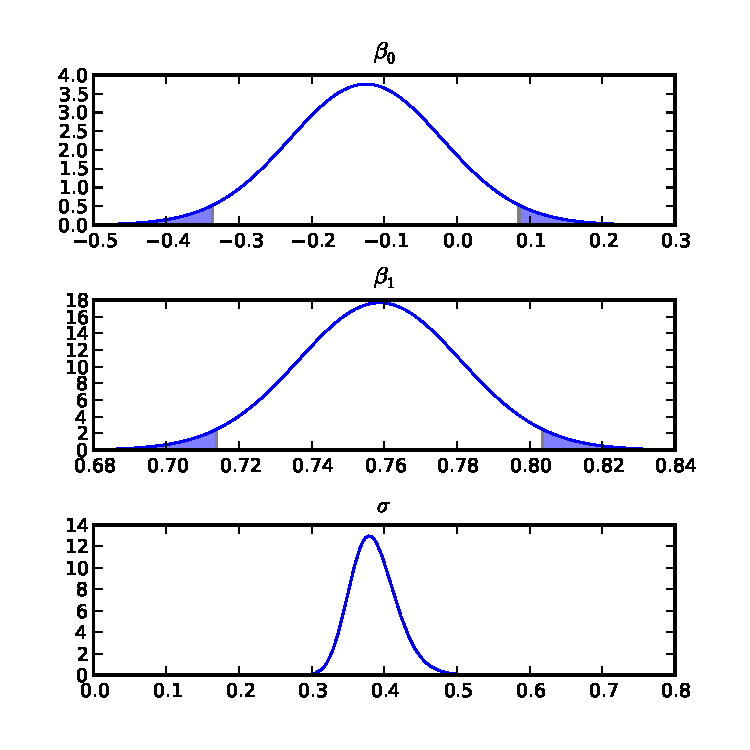
\includegraphics[width=9.5cm]{mpdreg.pdf}
  \end{center}
\caption{Marginal posterior density plots for the regression coefficients in example 1.}
\label{Flo:mpd reg}
\end{figure}



\subsection{Example 2: Log-linear model}
\label{sub:Example-2:-Log-linear}

For the log-linear model, see \citet{GelmanCarlinSternRubin2004}, the
$i^{th}$ observation $y_{i}$, for $i=1,2,\dots,n$, is generated as
follows
\begin{equation}
  p(y_{i}|\mu_{i})=\frac{\mu_{i}^{y_{i}}\exp(-\mu_{i})}{\mu_{i}!},\label{eq:observation
    equation log linear model}
\end{equation} with \[
\log(\mu_{i})=\bm{x}_{i}^{T}\bm{\beta},\] where $\bm{x}_{i}^{T}$ is
the $i^{th}$row of the $\left(n\times k\right)$ matrix $\bm{X}.$

The joint posterior distribution for the unknown parameter
$\bm{\beta}$ is given by
\begin{equation}
  p(\bm{\beta}|\bm{y},\bm{X})\propto p(\bm{y}|\bm{\beta},\bm{X})\times
  p(\bm{\beta}),
\label{eq:post log_linear}
\end{equation} 
where $p(\bm{y}|\bm{\beta},\bm{X})$ is the joint \emph{pdf }for
$\bm{y}$ conditional on the $\bm{\beta}$ and $\bm{X}$, and
$p(\bm{\beta})$ denotes the prior \emph{pdf }for $\bm{\beta}.$ From
(\ref{eq:observation equation log linear model}) it is apparent that\[
p(\bm{y}|\bm{\beta},\bm{X})=\prod_{i=1}^{n}\frac{\mu_{i}^{y_{i}}\exp(-\mu_{i})}{\mu_{i}!}.\]
A \emph{priori }we assume that \[ \bm{\beta}\sim
N(\bm{\underline{\bm{\beta}}},\bm{V}^{-1}).\]

To sample from (\ref{eq:post log_linear}), a random walk MH algorithm
is implemented, where the candidate $\bm{\beta}^{*}$, at each
iteration, is sampled following \begin{equation} \bm{\beta}^{*}\sim
  N\left(\bm{\beta}^{j-1},\bm{\Omega}\right),\label{eq:candidate
    log-linear}\end{equation} where\[
\bm{\beta}^{0}=\bm{\beta}_{nls}=\arg\min\left(\bm{y}-\exp\left(\bm{X}\bm{\beta}\right)\right)^{2}\]
and\[
\bm{\Omega}^{-1}=-\sum_{i=1}^{n}\exp\left(\bm{x}_{i}^{T}\bm{\beta}_{nls}\right)\bm{x}_{i}\bm{x}_{i}^{T}.\]



\subsubsection{Example code: Bayesian estimation of the log-linear model}

The example code for \pkg{PyMCMC} uses two \proglang{Python}
libraries, \pkg{Numpy} and \pkg{Scipy}, which the user must have
installed to run the code.  The code for the program is as follows:


\begin{lstlisting}[basicstyle={\scriptsize},numbers=left]
import os
from numpy import random, loadtxt, hstack, ones, dot, exp, zeros, outer, diag
from numpy import linalg
from pymcmc.mcmc import MCMC, RWMH, OBMC
from pymcmc.regtools import BayesRegression
from scipy.optimize.minpack import leastsq
import pymcmc

datadir = os.path.join(os.path.dirname(pymcmc.__file__), 'data')

def minfunc(beta, yvec, xmat ):
    return yvec - Exp(dot(xmat, beta))

def prior(store):
    mu = zeros(store['beta'].shape[0])
    Prec = diag(0.005 * ones(store['beta'].shape[0]))
    return -0.5 * dot(store['beta'].transpose(), dot(Prec, store['beta']))

def logl(store):
    xbeta = dot(store['xmat'], store['beta'])
    lamb = exp(xbeta)
    return sum(store['yvec'] * xbeta - Lamb)

def posterior(store):
    return logl(store) + prior(store)

def llhessian(store, beta):
    nobs = store['yvec'].shape[0]
    kreg = store['xmat'].shape[1]
    lamb = exp(dot(store['xmat'], beta))
    sum = zeros((kreg, kreg))
    for i in xrange(nobs):
        sum = sum + lamb[i] * outer(store['xmat'][i], store['xmat'][i])
    return -sum

random.seed(12345)      

data = loadtxt(os.path.join(datadir,'count.txt'), skiprows = 1)
yvec = data[:, 0]
xmat = data[:, 1:data.shape[1]]
xmat = hstack([ones((data.shape[0], 1)), xmat])

data ={'yvec':yvec, 'xmat':xmat} 
bayesreg = BayesRegression(yvec, xmat)     

sig, beta0 = bayesreg.posterior_mean()
init_beta, info = leastsq(minfunc, beta0, args = (yvec, xmat))
data['betaprec'] =-llhessian(data, init_beta)
scale = linalg.inv(data['betaprec'])

samplebeta = RWMH(posterior, scale, init_beta, 'beta')
ms = MCMC(20000, 4000, data, [samplebeta], loglike = (logl, xmat.shape[1], 'yvec'))
ms.sampler()
ms.output(filename='example1c.out') 
ms.plot('beta', filename='ex_loglinear.pdf')

ms.CODAoutput('beta')
ms.plot('beta', elements = [0], plottypes ="trace", filename ="xx.pdf")
ms.plot('beta', elements = [0], plottypes ="density", filename ="xx.png")
ms.plot('beta', elements = [0], plottypes ="acf", filename ="yy.ps")


\end{lstlisting}


The code for the analysis of the log-linear model is used to
demonstrate an application of straight Metropolis Hastings based
algorithms.  A brief description of the code is as follows:
\begin{itemize}
\item Lines 1-7 import the required classes and functions that are
  used in the program.
\item Line 9 is used to obtain the path of the data if installed
  using \code{setup.py}. Note that this step will not be necessary for
  normal usage of \pkg{PyMCMC}.
\item Lines 11-12 defines a function, \code{minfunc}, which is
  required in the non-linear least squares routine.
\item Lines 14-17 defines a function that evaluates the log of the
  prior pdf for, $\bm{\beta}.$ As in the variable selection example,
  \code{store} is a \proglang{Python} dictionary used to store all the
  information of interest that needs to be accessed by functions that
  are called from the MCMC sampler. For example, on line 22 it can be
  seen that \code{store{[}'beta'{]}} provides access to the vector
  $\bm{\beta}.$ Note the name \code{`beta'} is specified on line 72
  when the class for the random walk MH algorithm is initialised.
\item Lines 19-22 defines the log-likelihood function.
\item Lines 24-25 defines a function that evaluates the log of the
  posterior pdf for $\bm{\beta}.$
\item Lines 27-34 defines a function that returns the hessian for the
  log-linear model.
\item The main program begins on line 36 with the command to set the
  random seed.
\item Lines 38-41 load the data, from which arrays $\bm{y}$
  (\code{yvec}) and $\bm{X}$ (\code{xmat}) are constructed.
\item Lines 43-44 use Bayesian regression to initialise the nonlinear
  least squares algorithm.
\item Lines 46-49 perform nonlinear least squares operation.
\item Line 51 initialises the class \code{RWMH}. 
\item Line 52 initialises the class \code{MCMC} . Note that the
  sampling algorithm will be run for 20000 iterations and the first
  4000 will be discarded. The MCMC scheme has only one block and is a
  MH sampling scheme.
\item Line 53 runs the sampling scheme.
\item Lines 54-55 produce output.
\item Lines 57-60 demonstrate an example of how to produce CODA output
  and different ways in which plotting may be produced.
\end{itemize}

\subsubsection{Analysis}

The data analysed in this example are the number of nutgrass shoots
counted, in randomly scattered quadrats, at weekly intervals, during
the growing season. A log linear model is used; \begin{equation}
  \log(\mbox{count})=\beta_{0}+\beta_{1}\mbox{week}\end{equation}
where the intercept, $\beta_{0}$, is expected to be positive in value,
as nutgrass is always present in this study site, and $\beta_{1}$ is
also expected to be positive as the population of nutgrass increases
during the growing season.

\begin{verbatim}

--------------------------------------------------------

The time (seconds) for the Gibbs sampler =  7.47
Number of blocks in Gibbs sampler =  1

                mean        sd       2.5%     97.5%    IFactor
   beta[0]      1.14    0.0456       1.05      1.23       13.5
   beta[1]     0.157   0.00428      0.148     0.165       12.2
Acceptance rate  beta  =  0.5625
BIC =  -7718.074
Log likelihood =  3864.453

\end{verbatim}

It can be seen from the output that estimation is very fast (7.3
seconds), and that both $\beta_{0}$ and $\beta_{1}$ are positive
values, with $\hat{\beta}_{0}$ = 1.14 {[}1.05, 1.23{]} and
$\hat{\beta}_{1}$ = 0.157 {[}0.149, 0.165{]}. The marginal posterior
densities of these estimates (Figure 2) confirm that both estimates
are far from zero.

The ACF plots (Figure 2) and low inefficiency factors (see
\citet{ChibGreenberg1996} for details on inefficiency factors) of 12.6
($\hat{\beta}_{0}$) and 11.4 ($\hat{\beta}_{1}$) show that
autocorrelation in the sample is relatively low for an MCMC sampler. %
\begin{figure}[t!]
  \begin{center}
    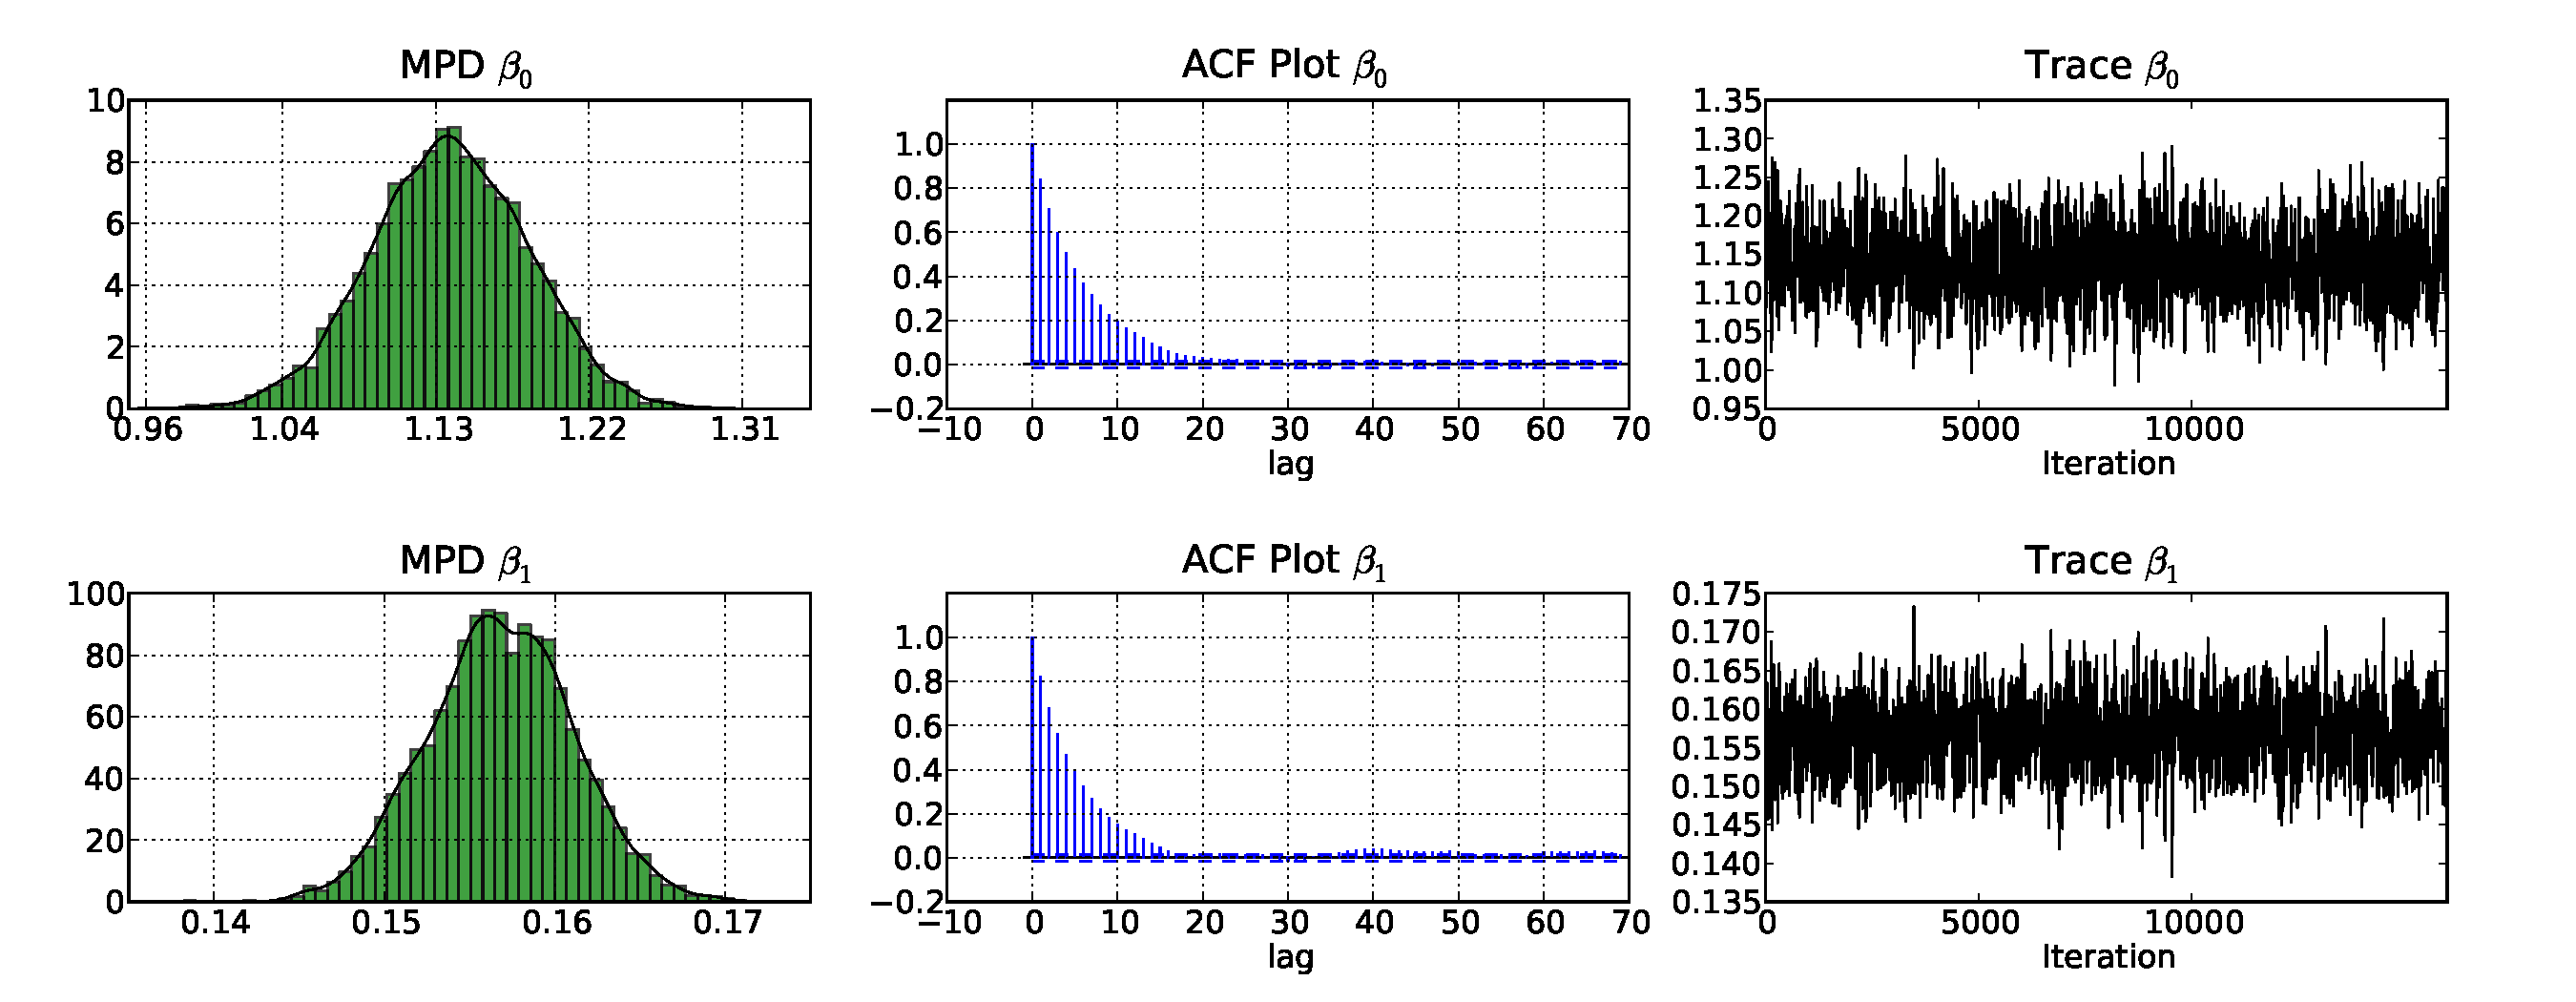
\includegraphics[width=16cm]{ex_loglinear.pdf}
  \end{center}
\caption{Plots of the marginal posterior density, autocorrelation and trace
plots for the MCMC estimation of the log linear model in example 2.}

\end{figure}

\subsection{Example 3: First order autoregressive regression}
\label{sub:Example-3:-First}

The linear regression model, with first order autocorrelated serial
correlation in the residuals, see \citet{Zellner1971} is defined such
that the $t^{th}$ observation, $y_{t},$ for
$t=1,2,\dots,n,$
\begin{equation}
  y_{t}=\bm{x}_{t}^{T}\bm{\beta}+\varepsilon_{t},\label{eq:observation
    ar}
\end{equation} 
with
\begin{equation}
  \varepsilon_{t}=\rho\varepsilon_{t-1}+\nu_{t};\,\,\,\nu_{t}\sim
  i.i.d.N(0,\sigma^{2}),
\label{eq:error ar}
\end{equation} where
\textbf{$\bm{x}_{t}$} is a $\left(k\times1\right)$ vector of
regressors, $\bm{\beta}$ is a $\left(k\times1\right)$ vector of
regression coefficients, $\rho$ is a damping parameter and $\nu_{t}$
is an independent identically normally distributed random variable
with a mean of 0 and a variance of $\sigma^{2}.$ Under the assumption
the the process driving the errors are stationary, that is $|\rho|<1,$
and assuming that the process has been running since time immemorial
then (\ref{eq:observation ar}) and (\ref{eq:error ar}) can be
expressed as

\begin{equation}
\bm{y}=\bm{X}\bm{\beta}+\bm{\varepsilon};\,\,\,\,\bm{\varepsilon}\sim N\left(\bm{0},\kappa^{-1}\bm{\Omega^{-1}}\right),\label{eq:observation2 ar}\end{equation}
 where \[
\bm{\Omega}=\left[\begin{array}{cccccc}
1 & -\rho & 0 & 0 & \cdots & 0\\
-\rho & 1+\rho^{2} & -\rho & 0 & \ddots & 0\\
0 & -\rho & 1+\rho^{2} & \ddots & \ddots & \vdots\\
0 & 0 & \ddots & \ddots & -\rho & 0\\
\vdots & \vdots & \ddots & -\rho & 1+\rho^{2} & -\rho\\
0 & 0 & \cdots & 0 & -\rho & 1\end{array}\right].\]
 Further, if we factorise $\bm{\Omega}=\bm{L}\bm{L}^{T},$ using the
Cholesky decomposition, it is straightforward to derive $\bm{L},$
where\[
\bm{L}=\left[\begin{array}{cccccc}
1 & -\rho & 0 & 0 & \cdots & 0\\
0 & 1 & -\rho & \ddots & \ddots & 0\\
0 & 0 & \ddots & \ddots & \ddots & \vdots\\
\vdots & \ddots & \ddots & \ddots & \ddots & 0\\
\vdots & \ddots & \ddots & \ddots & 1 & -\rho\\
0 & 0 & \cdots & \cdots & 0 & \sqrt{1-\rho^{2}}\end{array}\right].\]
 Pre-multiplying (\ref{eq:observation2 ar}), by $\bm{L}$ gives\begin{equation}
\bm{\tilde{y}}=\bm{\tilde{X}}\bm{\beta}+\bm{\tilde{\varepsilon}},\label{eq:trans_obs_ar}\end{equation}
 where $\bm{\tilde{y}}=\bm{L}^{T}\bm{y}$, $\bm{\tilde{X}}=\bm{L}^{T}\bm{X}$
and $\tilde{\bm{\varepsilon}}=\bm{L}^{T}\bm{\varepsilon}.$ Note that
$\bm{\varepsilon}\sim N(0,\kappa^{-1}\bm{I})$.

The joint posterior distribution for full set of unknown parameters
is
\begin{equation} p(\bm{\beta},\kappa,\rho|\bm{y})\propto
  p(\bm{y}|\bm{\beta},\kappa,\rho)\times p(\bm{\beta},\kappa)\times
  p(\rho),\label{eq:post_ar}
\end{equation} where
$p(\bm{y}|\bm{\beta},\kappa,\rho)$ is the joint \emph{pdf} of $\bm{y}$
conditional on $\bm{\beta},$ $\kappa,$ and $\rho$,
$p(\bm{\beta},\kappa)$ is the joint prior \emph{pdf} for $\bm{\beta}$
and $\kappa,$ and $p(\rho)$ denotes the prior density function for
$\rho.$ The likelihood function, which is defined following
(\ref{eq:observation ar}) and (\ref{eq:error ar}) is defined as
follows
\begin{eqnarray}
  p(\bm{y}|\bm{\beta},\kappa,\rho) & \propto & \kappa^{n/2}|\bm{\Omega}|^{1/2}\exp\left\{ -\frac{\kappa}{2}\left(\bm{y}-\bm{X}\bm{\beta}\right)^{T}\bm{\Omega}\left(\bm{y}-\bm{X}\bm{\beta}\right)\right\} \nonumber \\
  & = & \kappa^{n/2}|\bm{\Omega}|^{1/2}\exp\left\{ -\frac{\kappa}{2}\left(\tilde{\bm{y}}-\tilde{\bm{X}}\bm{\beta}\right)^{T}\left(\tilde{\bm{y}}-\tilde{\bm{X}}\bm{\beta}\right)\right\} .\nonumber \\
  & = & \kappa^{n/2}\left(1-\rho^{2}\right)^{1/2}\exp\left\{
    -\frac{\kappa}{2}\left(\tilde{\bm{y}}-\tilde{\bm{X}}\bm{\beta}\right)^{T}\left(\tilde{\bm{y}}-\tilde{\bm{X}}\bm{\beta}\right)\right\}
  .
  \label{eq:Likelihood AR1}
\end{eqnarray} 
For the analysis a normal-gamma prior is assumed for $\bm{\beta}$ and
$\kappa$, such that
\begin{equation} \bm{\beta}|\kappa\sim
  N\left(\underline{\bm{\beta}},\kappa^{-1}\right),\,\,\,\,\,\kappa\sim
  G\left(\frac{\underline{\nu}}{2},\frac{\underline{S}}{2}\right).
  \label{eq:prior
    beta AR1}
\end{equation} It follows from (\ref{eq:Likelihood AR1})
and (\ref{eq:prior beta AR1}) that sampling $\bm{\beta}$ and $\kappa$
conditional on $\rho$ is simply equivalent to sampling from a linear
regression model with a normal-gamma prior. A beta prior is assumed
for $\rho$ there by restricting the autocorrelation of the time series
to be both positive and stationary. Specifically\[
\rho\sim\mathcal{B}e\left(\alpha,\beta\right).\]

A MCMC sampling scheme, for the posterior distribution in
(\ref{eq:post_ar}), defined at iteration $j$ is as follows:
\begin{enumerate}
\item Sample $\bm{\beta}^{(j)},\kappa^{(j)}$ from
  $p(\bm{\beta},\kappa|\bm{y},\rho^{(j-1)}).$
\item Sample $\rho^{(j)}$ from $p(\rho|\bm{y},\bm{\beta},\kappa).$
\end{enumerate}

\subsubsection{Code: Example linear regression model with first order
  autocorrelation in the errors}

The example code for the linear regression model, with first order
autocorrelation in the errors uses the \proglang{Python} libraries
\pkg{Numpy}, \pkg{Scipy} and \pkg{Pysparse}. The code is used to
analyse simulated data.


\begin{lstlisting}[basicstyle={\scriptsize},numbers=left,tabsize=4]
from numpy import random, ones, zeros, dot, hstack, eye, log
from scipy import sparse
from pysparse import spmatrix
from pymcmc.mcmc import MCMC, SliceSampler, RWMH, OBMC, MH, CFsampler
from pymcmc.regtools import BayesRegression 

def simdata(nobs, kreg):
    xmat = hstack((ones((nobs, 1)), random.randn(nobs, kreg - 1)))
    beta = random.randn(kreg)
    sig = 0.2
    rho = 0.90
    yvec = zeros(nobs)
    eps = zeros(nobs)
    eps[0] = sig**2/(1.-rho**2)
    for i in xrange(nobs - 1):
        eps[i + 1] = rho * eps[i] + sig * random.randn(1)
    yvec = dot(xmat, beta) + eps
    return yvec, xmat

def calcweighted(store):
    nobs = store['yvec'].shape[0]
    store['Upper'].put(-store['rho'], range(0, nobs - 1), range(1, nobs))
    store['Upper'].matvec(store['yvec'], store['yvectil'])
    for i in xrange(store['xmat'].shape[1]):
        store['Upper'].matvec(store['xmat'][:, i], store['xmattil'][:, i])

def WLS(store):
    calcweighted(store)
    store['regsampler'].update_yvec(store['yvectil'])
    store['regsampler'].update_xmat(store['xmattil'])
    return store['regsampler'].sample()

def loglike(store):
    nobs = store['yvec'].shape[0]
    calcweighted(store)
    store['regsampler'].update_yvec(store['yvectil'])
    store['regsampler'].update_xmat(store['xmattil'])
    return store['regsampler'].loglike(store['sigma'], store['beta'])

def prior_rho(store):
    if store['rho'] > 0. and store['rho'] < 1.0:
        alpha = 1.0
        beta = 1.0
        return (alpha - 1.) * log(store['rho']) + (beta - 1.) * log(1.-store['rho'])
    else:
        return -1E256

def post_rho(store):
    return loglike(store) + prior_rho(store)

def gencand(store):
    return store['rho'] + 0.02 * random.randn(1)[0]

def probcandgprev(store):
    res = store['rho'] - Store['previous_rho']
    return -0.5/(0.02**2) * res**2

def probprevgcand(store):
    return probcandgprev(store)

random.seed(12345)
nobs = 1000
kreg = 3

yvec, xmat = simdata(nobs, kreg)

priorreg = ('g_prior', zeros(kreg), 1000.0)
regs = BayesRegression(yvec, xmat, prior = priorreg)

data ={'yvec':yvec, 'xmat':xmat, 'regsampler':regs}
U = spmatrix.ll_mat(nobs, nobs, 2 * nobs - 1)
U.put(1.0, range(0, nobs), range(0, nobs))
data['yvectil'] = zeros(nobs)
data['xmattil'] = zeros((nobs, kreg))
data['Upper'] = U

bayesreg = BayesRegression(yvec, xmat)
sig, beta = bayesreg.posterior_mean()

simsigbeta = CFsampler(WLS, [sig, beta], ['sigma', 'beta'])
scale = 0.002                       
rho = 0.9
simrho = SliceSampler([post_rho], 0.1, 5, rho, 'rho')
blocks = [simrho, simsigbeta]
loglikeinfo = (loglike, kreg + 2, 'yvec')
ms = MCMC(10000, 2000, data, blocks, loglike = loglikeinfo)
ms.sampler()
ms.output()
ms.plot('rho', filename ='rho')
ms.CODAoutput(parameters = ['rho'])
\end{lstlisting}


A brief description of the code above is as follows:
\begin{itemize}
\item Lines 1-5 import the specific functions and classes that are
  used in the analysis.
\item Lines 7-18 define a function that is used to produce the
  simulated data.
\item Lines 20-25 define a function that calculates $\tilde{\bm{y}}$
  and $\bm{\tilde{X}}.$ Note that line 22 updates $\bm{L}^{T}$ based
  on the latest iteration in the MCMC scheme. Note that $\bm{L}^{T}$
  is stored in the \proglang{Python} dictionary \code{store} and is
  accessed using the key \code{`Upper'}. It is stored in sparse matrix
  format using the library \pkg{Pysparse}.
\item Lines 27-31 define a function that is used to sample
  $\bm{\beta},$ from its conditional posterior distribution.
\item Lines 33-38 define a function that evaluates the log-likelihood
\item Lines 40-46 define the log of the prior pdf for $\rho$.
\item Lines 48-49 define a function that evaluates the log of the
  posterior pdf for $\rho.$
\item Lines 51 to 59 define functions that can be used to demonstrate
  the generic MH algorithm.
\item The main program begins with the command to set the random seed
  on line 61.
\item Lines 67-68 use g-prior for the regression coefficients.
\item Lines 70-75 construct the \proglang{Python} dictionary data,
  which is used to store information that will be passed to functions
  that are called from the MCMC sampler.
\item Lines 77-78 to use Bayesian regression to initialise the MCMC sampler.
\item Line 80 initialises the class instance \code{simsigbeta}, which is
used to jointly sample $\sigma$ and $\bm{\beta}.$ 
\item Line 83 provides an example of how to set up \pkg{PyMCMC} to
  sample $\rho$ using the Slice Sampler. This is the method that is
  used in the analysis below. Other algorithms which could be used
  here to simulate $\rho$ include RWMH, OBMC and generic MH.
\item Line 84 constructs a \proglang{Python} list that contain the
  class instances that define the MCMC sampler. In particular, it
  implies that the MCMC sampler consists of two blocks. Further,
  $\rho$ will be the first element sampled in the MCMC scheme.
\item Line 86 initialises \code{MCMC}. The MCMC sampler is run for
  8000 iterations and the first 2000 iterations are discarded in this
  instance.
\item Line 87 runs the sampler.
\item Lines 88-90 produce output from the MCMC sampler.
\end{itemize}

\subsubsection{Output}

\begin{verbatim}

The time (seconds) for the Gibbs sampler =  27.72
Number of blocks in Gibbs sampler =  2

                mean        sd       2.5%     97.5%    IFactor
   beta[0]    -0.523    0.0716     -0.653    -0.373        3.5
   beta[1]      1.85   0.00508       1.84      1.86       3.56
   beta[2]     0.455   0.00505      0.445     0.465       3.75
     sigma     0.217   0.00489      0.207     0.226        3.5
       rho     0.901    0.0155      0.872     0.932       3.67

Acceptance rate  beta  =  1.0
Acceptance rate  sigma  =  1.0
Acceptance rate  rho  =  1.0
BIC =  [-331.398]
Log likelihood =  [ 182.969]

\end{verbatim}

The analysis is conducted on a simulated data set, with 1000
observations and 3 regressors. The MCMC sampler is run for 10000
iterations and the first 2000 are discarded. The total time of
estimation is approximately 35 seconds. From the inefficiency factors
it is clear that the algorithm is very efficient.

%
\begin{figure}[t!]
\label{Flo:AR1}
\begin{center}
  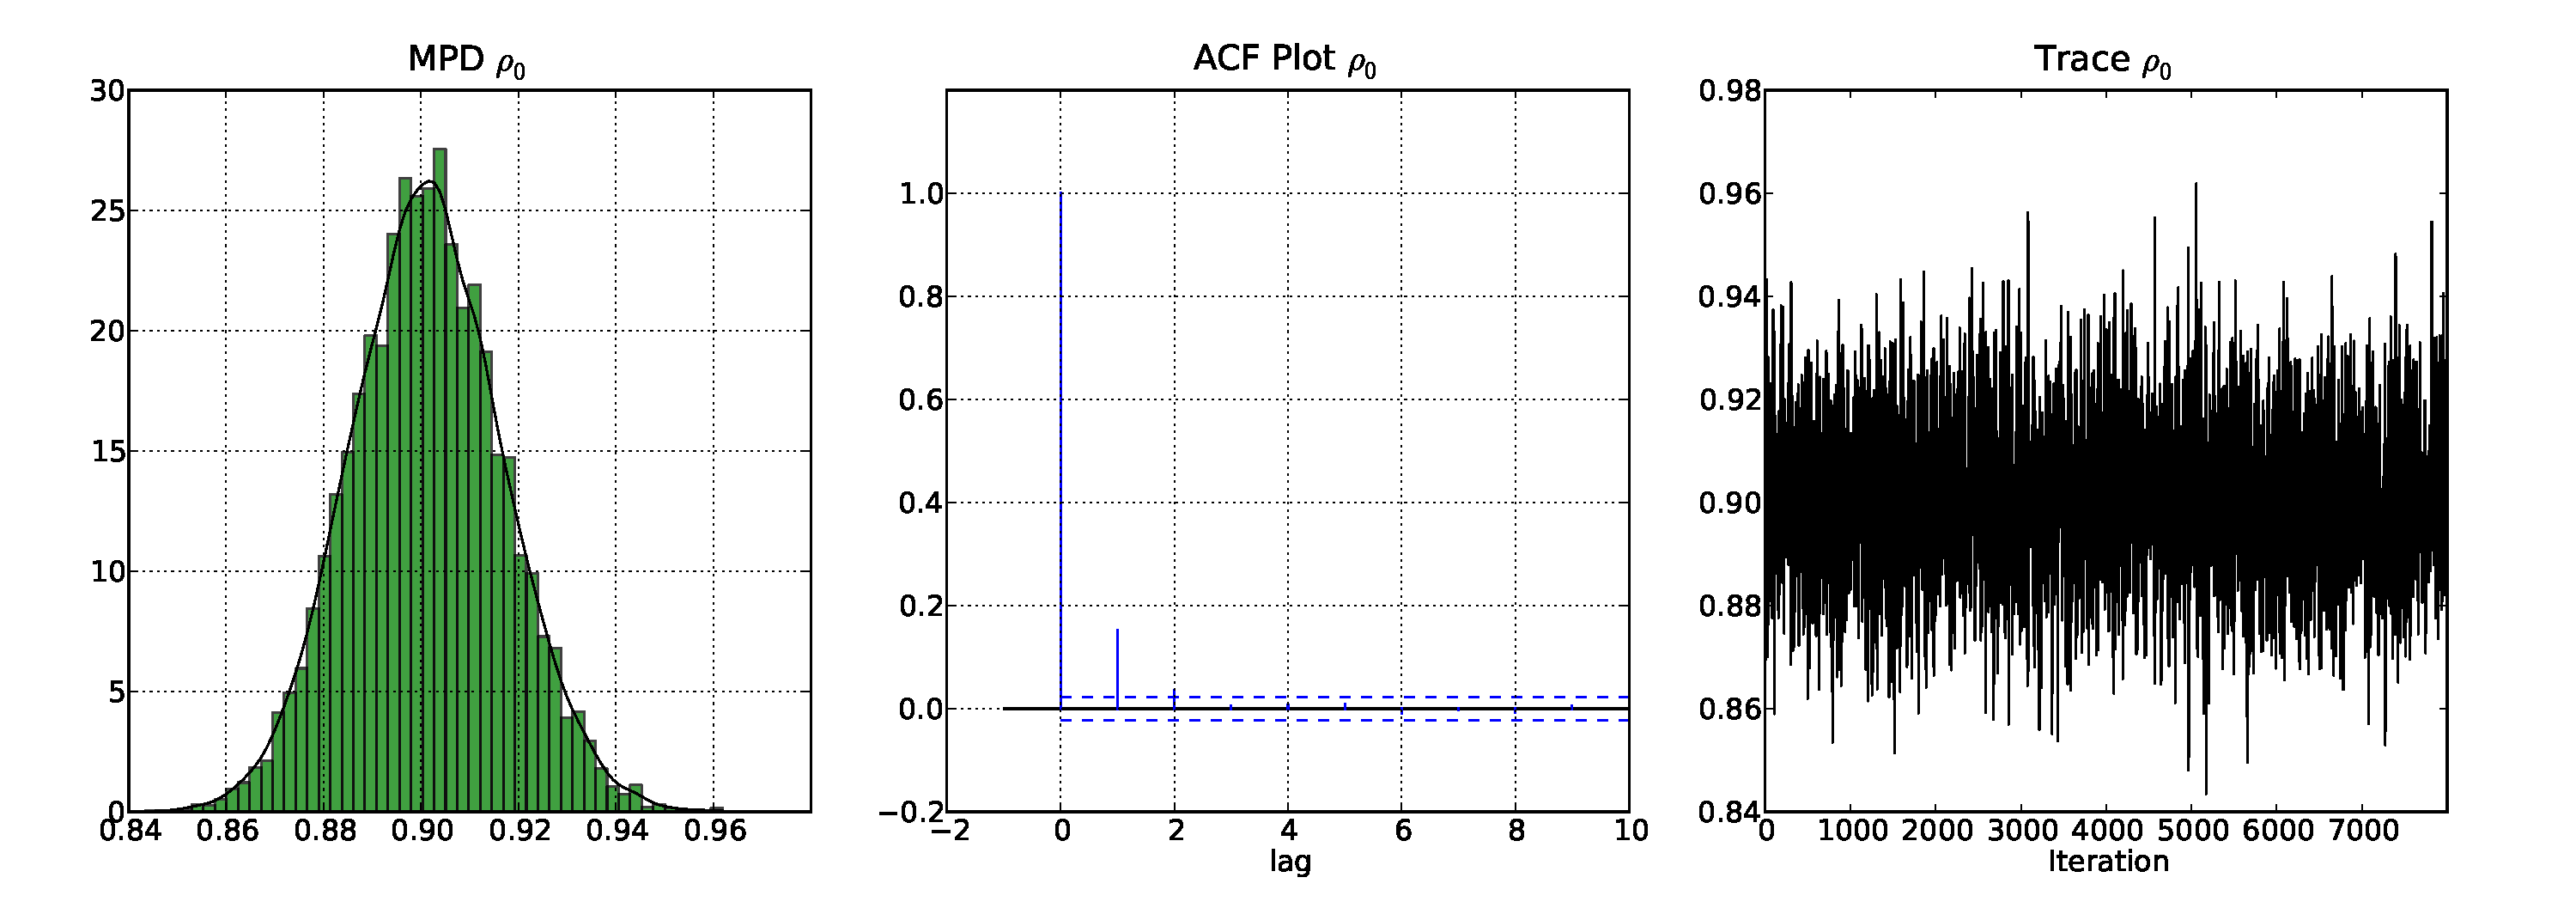
\includegraphics{rho.pdf}
\end{center}
\caption{Marginal posterior density, autocorrelation function and trace plot
based on the MCMC analysis for example 3.}

\end{figure}


Figure \ref{Flo:AR1} plots the marginal posterior density, autocorrelation
plot and the trace plot for the iterates. 


\section[Using PyMCMC  efficiently]{Using \pkg{PyMCMC}  efficiently}
\label{sec:Using-PyMCMC-efficiently}

The fact that MCMC algorithms rely on a large number of iterations to
achieve reasonable results and are often implemented on very large
problems, limits the practioners choice of a suitable environment, in
which they can implement efficient code. This efficiency comes through
an understanding of what makes a simulation efficient MCMC sampler,
and also the ability to produce computationally efficient code.
Interestingly, the two are related. To achieve both simulation and
computationally efficient code in MCMC samplers it is often extremely
important that large numbers of parameters are sampled in blocks,
rather than the alternative of a single move sampler. From the
perspective of simulation efficiency it is well known that indvidually
sampling correlated parameters induces correlation in the resultant
Markov chain and thus leads to a poorly mixing sampler. A classic
example in the literature are using \emph{simulation smoothers }to
jointly sample the state vector in a state space model; see for
example \citet{CarterKohn1994} and \citet{deJongShepard1995}.  Whilst
implementing a simulation smoother is required to achieve simulation
efficient code, the sequential nature of their implementation often
renders higher level languages impractical for large problems and thus
forces the analyst to write their entire code in a lower level
language. This is an inefficient use of time as usually only a small
percentage of code needs to be optimised. This drawback is easily
circumvented in \pkg{PyMCMC} as \proglang{Python} makes it easy to use
a lower level language to write the specialised module and use the
function directly from \proglang{Python}. This ensures \pkg{PyMCMC}'s
modules can be used for rapid development from \proglang{Python} and
lower level languages are only resorted to when necessary.

This section aims to provide guidelines for producing efficient code
with \pkg{PyMCMC}. We discuss alternative external libraries that are
available to the user for producing efficient code using \pkg{PyMCMC}.
Despite the ease of writing specialised modules this should not be the
first resort of the user. Instead, one should ensure that the
\proglang{Python} code is as efficient as possible using the resources
available with \proglang{Python}.

Arguably, the first thing the user of \pkg{PyMCMC} should concentrate
on when optimising their \pkg{PyMCMC} code is to ensure they use as
many inbuilt functions and libraries as possible. As most high
performance libraries are written in \proglang{C} or
\proglang{Fortran} this ensures that computationally expensive
procedures are computed using code from compiled languages.
\proglang{Python} users, and hence \pkg{PyMCMC} users, have an
enormous resource of Scientific libraries available to them as a
result of the popularity of \proglang{Python} in the scientific
community. Two of the most important libraries for most users will
quite possibly be \pkg{Numpy} and \pkg{Scipy}. Making use of such
libraries is one of the best ways of avoiding large loops in
procedures that are called from the MCMC sampler. If a large loop is
used inside a function that is called from inside the MCMC sampler
then this could mean that a large proportion of the total computation
is being done by \proglang{Python}, rather than a library that was
generated from optimised compiled code. This can have a dramatic
effect on the total computation time. As a simple and somewhat trivial
example we modify Example \ref{sub:Example-2:-Log-linear} so that a
loop is explicitly used to calculate the log likelihood.




\begin{lstlisting}[basicstyle={\scriptsize}]
def logl(store):
    suml=0.0
    for i in xrange(store['yvec'].shape[0]):
        xbeta=dot(store['xmat'][i,:],store['beta'])
        suml=suml+store['yvec'][i] * xbeta - Exp(xbeta)
    return suml
\end{lstlisting}


Whilst the two functions to calculate the log-likelihood are
mathematically equivalent, the one with the explicit loop is
substantially slower.  Specifically, the time taken for the MCMC
sampler went from 7.3 seconds to 130.19 seconds. As such, this minor
modification leads to an approximate 18-fold decrease in the speed of
the program.

If the use of an an inbuilt function is not possible and the time
taken from the program is unacceptable then there are several
alternative solutions available to the user. One such solution is to
use the package \pkg{Weave}, which is a part of the \pkg{Scipy}
library, to write inline \proglang{C} code which will accelerate the
problem area in the code. An example is given below.


\begin{lstlisting}[basicstyle={\scriptsize}]
def logl(store):
    code = """     
		double sum = 0.0, xbeta;
		for(int i=0; i<nobs; i++){
			xbeta = 0.0;
			for(int j=0; j<kreg; j++){xbeta += xmat[i+j*kreg] * beta[j];}
			sum += yvec[i] * xbeta - Exp(xbeta);
		}     
		return_val = sum;
    """
    yvec = store['yvec']
    xmat = store['xmat']
	nobs, kreg = xmat.shape
	beta = store['beta']
    return weave.inline(code,['yvec','xmat', 'beta','nobs','kreg'],\ 
                       compiler='gcc')
\end{lstlisting}


The total time taken for weave version is 4.33 seconds. The reason for
the speed increase over the original version that uses \pkg{Numpy}
functions is the weave version avoids the construction of temporary
matrices that are typically a by product of overloaded operators.

Another alternative, which is our preferred approach, is to use the
\proglang{Python} module \pkg{F2py}; see \citet{F2PY} for further
details. \pkg{F2py} allows for the seamless integration of
\proglang{Fortran} and \proglang{Python} code. Following on using the
same trivial example we use the following \proglang{Fortran77} code.
This example requires that the user the have basic linear algebra
subprograms (\pkg{BLAS}) and and preferable also the automatically
tuned
linear algebra software (\pkg{ATLAS}).\\
 
\begin{lstlisting}[basicstyle={\scriptsize}]
c     fortran 77 code used to calculate the likelihood of a log
c     linear model. Subroutine uses BLAS.

      subroutine logl(xb,xm,bv,yv,llike,n,k)
      implicit none
      integer n, k, i, j
      real*8 xb(n),xm(n,k), bv(k), yv(n), llike
      real*8 alpha, beta

cf2py intent(in,out) logl
cf2py intent(in) yv
cf2py intent(ini bv
cf2py intent(in) xmat 
cf2py intent(in) xb 

      alpha=1.0
      beta=0.0
      call dgemv('n',n,k,alpha,xm,n,bv,1,beta,xb,1)

      llike=0.0
      do i=1,n
          llike=llike+yv(i)*xb(i)-exp(xb(i))
      enddo
      end
\end{lstlisting}


The code is compiled with the command (Note: see the following
subsection if you are a Microsoft Windows user, this command is for
UNIX type environments such as Linux and OSX): In UNIX type
environments, such as Linux and OSX the code is compiled with the
following command (Windows users see Section \ref{CompilingWindows})

f2py -c loglinear.f -m loglinear -lblas -latlas

then called from \proglang{Python} as follows


\begin{lstlisting}[basicstyle={\scriptsize}]
import loglinear
\end{lstlisting}


The loglinear library must be imported to be accessible and is done as
above. The log-likelihood function is then modified as follows


\begin{lstlisting}[basicstyle={\scriptsize},numbers=left]
def logl(store):
	loglike=array(0.0)     
	return loglinear.logl(store['xb'],store['xmatf'], store['beta'],store['yvec'],loglike)
    
\end{lstlisting}


The code in example1c.py is further modified by inserting the
following code before line 64 in the original program.


\begin{lstlisting}[basicstyle={\scriptsize}]
data['xb']=zeros(yvec.shape[0])
data['xmatf']=asfortranarray(xmat)
\end{lstlisting}


The array \code{data{[}`xb'{]}} is a work array used for the
calculation of $\bm{X}\bm{\beta}.$ It is stored in in the
\proglang{Python} dictionary \code{data}, so it is only created once
rather that each time the function \code{logl} is called. The second
array \code{data{[}`xmatf'{]}} stores $\bm{X}$ in column major order,
which is what is used in \proglang{Fortran}, rather than the
\proglang{Python} default, which is row major order the default for
the \proglang{C} programming language. If \code{store{[}`xmat'{]}} is
passed to the function \code{loglinear.logl} then f2py will
automatically produce a copy and convert it to column major order each
time the function \code{logl} is called.

The total time for the MCMC sampler when using f2py is 4.03 seconds.
This is slightly faster that the version that uses Weave, where most
likely the small gain can be attributed to the use of ATLAS.

The user has many other choices available to them for writing
specialised extension modules. For example, if it is the preference of
the user it is not much more difficult to use \pkg{F2py} to compile
procedures written in \proglang{C}, which then can be used directly
from \proglang{Python}. Another popular library that can be used to
marry \proglang{C}, as well as \proglang{C++}, code with
\proglang{Python} is \pkg{SWIG}. In our opinion \pkg{SWIG} is more
difficult than \pkg{f2py} for complicated examples. The user may also
opt to manually call \proglang{C} and \proglang{C++} routines using
\proglang{Python} and \pkg{Numpy}'s \proglang{C} application
interface. Another option for \proglang{C++} users is to use
\pkg{Boost} \proglang{Python}. These alternative approaches are beyond
the scope of this paper.


\subsection{Compiling code in Windows}
\label{CompilingWindows}

The previous section described how one might go about using
\pkg{PyMCMC} efficiently. To do this, access to a compiler is
necessary. Under most flavours of UNIX, this should pose no problem,
but under Microsoft Windows this can be more difficult. This section
provides some brief guidelines to an approach we found workable under
Windows.

In order to run \pkg{PyMCMC}, \proglang{Python}, \pkg{Numpy} and
\pkg{Scipy} are all required, but to have a reasonable developer
experience under Windows, we suggest a few additional packages, all of
which are freely available:
\begin{itemize}
\item \pkg{mingw} (http://www.mingw.org/) which provides, among other
  things, the GNU compler suite. The user should choose at least
  \pkg{gcc} and \pkg{g++}.
\item \pkg{msys} (http://www.mingw.org/wiki/MSYS) which provides a set
  of GNU utilities commonly found on Linux. This will make building
  and compiling code more manageable under Windows.
\item \pkg{ipython} (http://ipython.scipy.org/moin/), an interactive
  interface to \proglang{Python}, which can be used as an alternative
  to the idle interface that is distributed with \proglang{Python}.
\item \pkg{pyreadline}
  (http://ipython.scipy.org/moin/PyReadline/Intro), which provides
  Windows readline capabilities for IPython.
\item \pkg{gfortran} (http://gcc.gnu.org/wiki/GFortranBinaries), which
  provides a native Windows \proglang{Fortran} compiler.
\end{itemize}
Once these additional utilities are installed, it should be possible
to compile code in different languages. To test that Weave works as
expected, make sure that the \pkg{mingw} bin directory is in your
path, and try the following code:


\begin{lstlisting}[basicstyle={\scriptsize}]
import scipy.weave 
a=100 
scipy.weave.inline('printf("a=%d\\n",a);',['a'],verbose=1)
\end{lstlisting}


The output should be similar to:


\begin{lstlisting}[basicstyle={\scriptsize}]
In [4]: scipy.weave.inline('printf("a=%d\\n",a);',['a'],verbose=1)
<weave: compiling>
No module named msvccompiler in numpy.distutils; trying from distutils
Compiling code...
Found executable c:\mingw\bin\g++.exe
finished compiling (sec):  2.73600006104
a=100
\end{lstlisting}


\pkg{F2py} requires a \proglang{Fortran} compiler. To set this up
under Windows, follow the instructions at
http://www.scipy.org/F2PY\_Windows, and make sure the simple example
provided works on your system. The examples presented above
additionally require \pkg{BLAS} or \pkg{ATLAS} to be available. This
can be built under windows (see instructions at
http://www.scipy.org/Installing\_SciPy/Windows, for example). To check
that \pkg{F2py} and ATLAS are installed correctly, save the following
code as, for example, blas\_eg.f90:


\begin{lstlisting}[basicstyle={\scriptsize}]
subroutine dgemveg()
  REAL*8 X(2, 3) /1.D0, 2.D0, 3.D0, 4.D0, 5.D0, 6.D0/
  REAL*8 Y(3) /2.D0, 2.D0, 2.D0/
  REAL*8 Z(2)
  CALL DGEMV('N', 2, 3, 1.D0, X, 2, Y, 1, 0.D0, Z, 1)
  PRINT *, Z
end subroutine dgemveg
\end{lstlisting}


Set the location of your ATLAS libraries appropriately, and ensure
that gfortran is in your path and compile. The following provides a
template:


\begin{lstlisting}[basicstyle={\scriptsize}]
ATLAS_LIB_DIR="/d/tmp/pymcmc_win_install/BUILDS/lib"
export PATH=${PATH}:/c/Program\ Files/gfortran/libexec/gcc/i586-pc-mingw32/4.6.0:/c/Program\ Files/gfortran/bin:/c/python26 
python /c/Python26/Scripts/f2py.py -c -m foo \
   --fcompiler=gfortran \
   blas_eg.f90 -L${ATLAS_LIB_DIR} -lf77blas -latlas -lg2c 
\end{lstlisting}


This should produce a \proglang{Python} dll (foo.pyd), which can be imported
into \proglang{Python}:


\begin{lstlisting}[basicstyle={\scriptsize}]
import foo
dir(foo) 
print foo.__doc__
foo.dgemveg() 
\end{lstlisting}

\section[PyMCMC interacting with R]{\pkg{PyMCMC} interacting with R}
\label{sec:PyMCMC-interacting-with}

There are many functions from the \proglang{R} statistical language
\citep{R} that can be useful in Bayesian analysis. The \pkg{RPy2}
\proglang{Python} library can be used to integrate \proglang{R}
functions into \pkg{PyMCMC} programs. These can be accessed in
\pkg{PyMCMC} through the \pkg{RPy2} \proglang{Python} library. As an
example, consider the Log linear model described in Section
\ref{sub:Example-2:-Log-linear}. The random walk MH requires the
specification of a candidate density function Equation (\ref{random
  walk candidate}) and an initial value. The R functions \texttt{glm
}and \texttt{summary.glm} can be used to set this to the maximum
likelihood estimate $\hat{\beta}$ and the unscaled estimated
covariance matrix of the estimated coefficients. The relevant code is
summarised below:


\begin{lstlisting}[basicstyle={\scriptsize},numbers=left,tabsize=4]
import rpy2.robjects.numpy2ri
from rpy2 import rinterface
import rpy2.robjects as robjects

def initial_values(yvec,xmat):
    ry = rinterface.SexpVector(yvec,rinterface.INTSXP)
    rx = rinterface.SexpVector(xmat[:,1:],rinterface.INTSXP)
    robjects.globalenv['y'] = ry
    robjects.globalenv['x'] = rx
    mod = robjects.r.glm("y~x", family="poisson")
    init_beta =  array(robjects.r.coefficients(mod))
    modsummary = robjects.r.summary(mod)
    scale = array(modsummary.rx2('cov.unscaled'))
    return init_beta,scale

random.seed(12345) 
data=loadtxt('count.txt',skiprows=1)
yvec=data[:,0]
xmat=data[:,1:data.shape[1]]
xmat=hstack([ones((data.shape[0],1)),xmat])

data={'yvec':yvec,'xmat':xmat} 

init_beta,scale=initial_values(yvec,xmat)

samplebeta=RWMH(posterior,scale,init_beta,'beta')
GS=Gibbs(20000,4000,data, [samplebeta],loglike=(logl,xmat.shape[1],'yvec'))
GS.sampler()
GS.CODAoutput(filename="loglinear_eg") 

\end{lstlisting}


It may also be useful to take advantage of the many MCMC analysis
functions in \proglang{R} and associated packages. To facilitate this,
\pkg{PyMCMC} includes a CODA
\citep{Rnews:Plummer+Best+Cowles+Vines:2006} output format which can
easily be read into\proglang{R}for further analysis. A sample
\proglang{R} session after \pkg{PyMCMC} might look like:


\begin{lstlisting}[basicstyle={\scriptsize},language=R,numbers=left]
library(coda)
aa <- Read.coda("loglinear_eg.txt","loglinear_eg.ind")
plot(aa)
summary(aa)
raftery.diag(aa)
xyplot(aa)
densityplot(aa)
acfplot(aa,lag.max=500)

\end{lstlisting}



\section{Conclusions}
\label{sec:Conclusions}

In this paper, we have described the \proglang{Python} software
package \pkg{PyMCMC}.  \pkg{PyMCMC} takes advantage of the flexibility
and extensibility of \proglang{Python} to provide the user with a code
efficient way of constructing MCMC samplers. The \pkg{PyMCMC} package
includes classes for the MCMC sampler MH, independent MH, random walk
MH, OBMC and slice sampling algorithms.  It also contains an inbuilt
module for Bayesian regression analysis.  We demonstrate \pkg{PyMCMC}
using an example of Bayesian regression analysis with stochastic
search variable selection, a log-linear model and also a time series
regression analysis with first order autoregressive errors. We
demonstrate how to optimise \pkg{PyMCMC} using \pkg{Numpy} functions,
inline \proglang{C} code using \pkg{Weave} and with
\proglang{Fortran77} using \pkg{F2py}, where necessary.  We further
demonstrate how to call \proglang{R} functions using \pkg{RPy2}.


\subsection*{Acknowledgements}

This research has been supported by an Australian Research Council
Linkage Grant; LP100100565. The code was primarily developed and
tested using Arch Linux http://www.archlinux.org/ and Kubuntu
http://www.kubuntu.org/.

\bibliography{chris}

\end{document}
